% Options for packages loaded elsewhere
\PassOptionsToPackage{unicode}{hyperref}
\PassOptionsToPackage{hyphens}{url}
%
\documentclass[
]{book}
\usepackage{amsmath,amssymb}
\usepackage{lmodern}
\usepackage{ifxetex,ifluatex}
\ifnum 0\ifxetex 1\fi\ifluatex 1\fi=0 % if pdftex
  \usepackage[T1]{fontenc}
  \usepackage[utf8]{inputenc}
  \usepackage{textcomp} % provide euro and other symbols
\else % if luatex or xetex
  \usepackage{unicode-math}
  \defaultfontfeatures{Scale=MatchLowercase}
  \defaultfontfeatures[\rmfamily]{Ligatures=TeX,Scale=1}
\fi
% Use upquote if available, for straight quotes in verbatim environments
\IfFileExists{upquote.sty}{\usepackage{upquote}}{}
\IfFileExists{microtype.sty}{% use microtype if available
  \usepackage[]{microtype}
  \UseMicrotypeSet[protrusion]{basicmath} % disable protrusion for tt fonts
}{}
\makeatletter
\@ifundefined{KOMAClassName}{% if non-KOMA class
  \IfFileExists{parskip.sty}{%
    \usepackage{parskip}
  }{% else
    \setlength{\parindent}{0pt}
    \setlength{\parskip}{6pt plus 2pt minus 1pt}}
}{% if KOMA class
  \KOMAoptions{parskip=half}}
\makeatother
\usepackage{xcolor}
\IfFileExists{xurl.sty}{\usepackage{xurl}}{} % add URL line breaks if available
\IfFileExists{bookmark.sty}{\usepackage{bookmark}}{\usepackage{hyperref}}
\hypersetup{
  pdftitle={COMP 4441 Final Project},
  pdfauthor={Emma Bright and Michael Santoro},
  hidelinks,
  pdfcreator={LaTeX via pandoc}}
\urlstyle{same} % disable monospaced font for URLs
\usepackage{color}
\usepackage{fancyvrb}
\newcommand{\VerbBar}{|}
\newcommand{\VERB}{\Verb[commandchars=\\\{\}]}
\DefineVerbatimEnvironment{Highlighting}{Verbatim}{commandchars=\\\{\}}
% Add ',fontsize=\small' for more characters per line
\usepackage{framed}
\definecolor{shadecolor}{RGB}{248,248,248}
\newenvironment{Shaded}{\begin{snugshade}}{\end{snugshade}}
\newcommand{\AlertTok}[1]{\textcolor[rgb]{0.94,0.16,0.16}{#1}}
\newcommand{\AnnotationTok}[1]{\textcolor[rgb]{0.56,0.35,0.01}{\textbf{\textit{#1}}}}
\newcommand{\AttributeTok}[1]{\textcolor[rgb]{0.77,0.63,0.00}{#1}}
\newcommand{\BaseNTok}[1]{\textcolor[rgb]{0.00,0.00,0.81}{#1}}
\newcommand{\BuiltInTok}[1]{#1}
\newcommand{\CharTok}[1]{\textcolor[rgb]{0.31,0.60,0.02}{#1}}
\newcommand{\CommentTok}[1]{\textcolor[rgb]{0.56,0.35,0.01}{\textit{#1}}}
\newcommand{\CommentVarTok}[1]{\textcolor[rgb]{0.56,0.35,0.01}{\textbf{\textit{#1}}}}
\newcommand{\ConstantTok}[1]{\textcolor[rgb]{0.00,0.00,0.00}{#1}}
\newcommand{\ControlFlowTok}[1]{\textcolor[rgb]{0.13,0.29,0.53}{\textbf{#1}}}
\newcommand{\DataTypeTok}[1]{\textcolor[rgb]{0.13,0.29,0.53}{#1}}
\newcommand{\DecValTok}[1]{\textcolor[rgb]{0.00,0.00,0.81}{#1}}
\newcommand{\DocumentationTok}[1]{\textcolor[rgb]{0.56,0.35,0.01}{\textbf{\textit{#1}}}}
\newcommand{\ErrorTok}[1]{\textcolor[rgb]{0.64,0.00,0.00}{\textbf{#1}}}
\newcommand{\ExtensionTok}[1]{#1}
\newcommand{\FloatTok}[1]{\textcolor[rgb]{0.00,0.00,0.81}{#1}}
\newcommand{\FunctionTok}[1]{\textcolor[rgb]{0.00,0.00,0.00}{#1}}
\newcommand{\ImportTok}[1]{#1}
\newcommand{\InformationTok}[1]{\textcolor[rgb]{0.56,0.35,0.01}{\textbf{\textit{#1}}}}
\newcommand{\KeywordTok}[1]{\textcolor[rgb]{0.13,0.29,0.53}{\textbf{#1}}}
\newcommand{\NormalTok}[1]{#1}
\newcommand{\OperatorTok}[1]{\textcolor[rgb]{0.81,0.36,0.00}{\textbf{#1}}}
\newcommand{\OtherTok}[1]{\textcolor[rgb]{0.56,0.35,0.01}{#1}}
\newcommand{\PreprocessorTok}[1]{\textcolor[rgb]{0.56,0.35,0.01}{\textit{#1}}}
\newcommand{\RegionMarkerTok}[1]{#1}
\newcommand{\SpecialCharTok}[1]{\textcolor[rgb]{0.00,0.00,0.00}{#1}}
\newcommand{\SpecialStringTok}[1]{\textcolor[rgb]{0.31,0.60,0.02}{#1}}
\newcommand{\StringTok}[1]{\textcolor[rgb]{0.31,0.60,0.02}{#1}}
\newcommand{\VariableTok}[1]{\textcolor[rgb]{0.00,0.00,0.00}{#1}}
\newcommand{\VerbatimStringTok}[1]{\textcolor[rgb]{0.31,0.60,0.02}{#1}}
\newcommand{\WarningTok}[1]{\textcolor[rgb]{0.56,0.35,0.01}{\textbf{\textit{#1}}}}
\usepackage{longtable,booktabs,array}
\usepackage{calc} % for calculating minipage widths
% Correct order of tables after \paragraph or \subparagraph
\usepackage{etoolbox}
\makeatletter
\patchcmd\longtable{\par}{\if@noskipsec\mbox{}\fi\par}{}{}
\makeatother
% Allow footnotes in longtable head/foot
\IfFileExists{footnotehyper.sty}{\usepackage{footnotehyper}}{\usepackage{footnote}}
\makesavenoteenv{longtable}
\usepackage{graphicx}
\makeatletter
\def\maxwidth{\ifdim\Gin@nat@width>\linewidth\linewidth\else\Gin@nat@width\fi}
\def\maxheight{\ifdim\Gin@nat@height>\textheight\textheight\else\Gin@nat@height\fi}
\makeatother
% Scale images if necessary, so that they will not overflow the page
% margins by default, and it is still possible to overwrite the defaults
% using explicit options in \includegraphics[width, height, ...]{}
\setkeys{Gin}{width=\maxwidth,height=\maxheight,keepaspectratio}
% Set default figure placement to htbp
\makeatletter
\def\fps@figure{htbp}
\makeatother
\setlength{\emergencystretch}{3em} % prevent overfull lines
\providecommand{\tightlist}{%
  \setlength{\itemsep}{0pt}\setlength{\parskip}{0pt}}
\setcounter{secnumdepth}{5}
\ifluatex
  \usepackage{selnolig}  % disable illegal ligatures
\fi
\usepackage[]{natbib}
\bibliographystyle{apalike}

\title{COMP 4441 Final Project}
\author{Emma Bright and Michael Santoro}
\date{2021-06-07}

\begin{document}
\maketitle

{
\setcounter{tocdepth}{1}
\tableofcontents
}
\hypertarget{introduction}{%
\chapter{Introduction}\label{introduction}}

\textbf{Purpose}

Wine is an alcoholic beverage made from fermented grape juice. \citet{wine_exactly_web} Generally, a wine's quality is determined by taste, smell, and visual tests performed by wine experts, sommeliers. These tests grade the wine on subjective measures: Acidity, Sweetness, Alcohol, Tannin and Aroma. Though these tests are subjective, there is overlap between the observation of these characteristics and a wine's physiochemical properties. For example, a wine's perceived acidity or tartness is based upon the pH of the wine and a wine's perceived sweetness is based upon the residual sugar of the wine.

The goal of our research is to determine:

Can we determine an accurate subjective rating of a wine based solely on its physicochemical properties?

\textbf{\emph{Why is this important?}}

An accurate predictive model for determining the quality of wine will enable small wineries and vineyards, especially those from less established wine regions, to more accurately price their inventory and ensure a better return on investment.

\textbf{Statistical or Analytical Method}

We will be using the the following statistical methods to create predictive models for quality of wine:

\begin{itemize}
\tightlist
\item
  Random Forest
\item
  K-Nearest Neighbor
\item
  Elastic Net Regression (LASSO and Ridge)
\end{itemize}

\hypertarget{descriptive-statistics}{%
\chapter{Descriptive Statistics}\label{descriptive-statistics}}

\hypertarget{dataset}{%
\section{Dataset}\label{dataset}}

The dataset utilized for our analysis was collected from the UCI Machine Learning Repository \citet{model_wine}. The dataset consists of 12 elements, 11 physiochemical properties and 1 subjective quality measurement, for both red and white Vinho Verde wine samples from Portugal.

\textbf{Read in Data}

\begin{Shaded}
\begin{Highlighting}[]
\NormalTok{redWine}\OtherTok{\textless{}{-}}\FunctionTok{read.table}\NormalTok{(}\StringTok{"data/winequality{-}red.csv"}\NormalTok{,}\AttributeTok{stringsAsFactors =} \ConstantTok{FALSE}\NormalTok{,}
                \AttributeTok{sep=}\StringTok{","}\NormalTok{,}\AttributeTok{header =} \ConstantTok{TRUE}\NormalTok{)}
\NormalTok{whiteWine}\OtherTok{\textless{}{-}}\FunctionTok{read.table}\NormalTok{(}\StringTok{"data/winequality{-}white.csv"}\NormalTok{,}\AttributeTok{stringsAsFactors =} \ConstantTok{FALSE}\NormalTok{,}
                \AttributeTok{sep=}\StringTok{";"}\NormalTok{,}\AttributeTok{header =} \ConstantTok{TRUE}\NormalTok{)}

\CommentTok{\# create a field that shows whether a wine is red or white based on initial }
\CommentTok{\# datasets}
\NormalTok{redWine}\SpecialCharTok{$}\NormalTok{type}\OtherTok{=}\StringTok{\textquotesingle{}red\textquotesingle{}}
\NormalTok{whiteWine}\SpecialCharTok{$}\NormalTok{type}\OtherTok{=}\StringTok{\textquotesingle{}white\textquotesingle{}}

\CommentTok{\# merge data}
\NormalTok{wine }\OtherTok{\textless{}{-}} \FunctionTok{rbind}\NormalTok{(redWine, whiteWine)}

\FunctionTok{str}\NormalTok{(wine)}
\end{Highlighting}
\end{Shaded}

\begin{verbatim}
## 'data.frame':    6497 obs. of  13 variables:
##  $ fixed.acidity       : num  7.4 7.8 7.8 11.2 7.4 7.4 7.9 7.3 7.8 7.5 ...
##  $ volatile.acidity    : num  0.7 0.88 0.76 0.28 0.7 0.66 0.6 0.65 0.58 0.5 ...
##  $ citric.acid         : num  0 0 0.04 0.56 0 0 0.06 0 0.02 0.36 ...
##  $ residual.sugar      : num  1.9 2.6 2.3 1.9 1.9 1.8 1.6 1.2 2 6.1 ...
##  $ chlorides           : num  0.076 0.098 0.092 0.075 0.076 0.075 0.069 0.065 0.073 0.071 ...
##  $ free.sulfur.dioxide : num  11 25 15 17 11 13 15 15 9 17 ...
##  $ total.sulfur.dioxide: num  34 67 54 60 34 40 59 21 18 102 ...
##  $ density             : num  0.998 0.997 0.997 0.998 0.998 ...
##  $ pH                  : num  3.51 3.2 3.26 3.16 3.51 3.51 3.3 3.39 3.36 3.35 ...
##  $ sulphates           : num  0.56 0.68 0.65 0.58 0.56 0.56 0.46 0.47 0.57 0.8 ...
##  $ alcohol             : num  9.4 9.8 9.8 9.8 9.4 9.4 9.4 10 9.5 10.5 ...
##  $ quality             : int  5 5 5 6 5 5 5 7 7 5 ...
##  $ type                : chr  "red" "red" "red" "red" ...
\end{verbatim}

The table above shows the structure of our dataset before any sort of data manipulation, munging, or cleaning.

\hypertarget{exploratory-analysis}{%
\section{Exploratory Analysis}\label{exploratory-analysis}}

\hypertarget{descriptive-statistics-1}{%
\subsection{Descriptive Statistics}\label{descriptive-statistics-1}}

In order to better understand our data set we performed some initial descriptive statistics. A descriptive statistic is a summary level statistic, such as mean or median, that describes a variable or feature of a dataset. Descriptive statistics is the processing of analyzing the descriptive statistic taken from your dataset. \citet{descrip_stat}

The table below shows descriptive statistic measurements for each of the variables in our dataset.

\begin{Shaded}
\begin{Highlighting}[]
\FunctionTok{stat.desc}\NormalTok{(wine)}
\end{Highlighting}
\end{Shaded}

\begin{verbatim}
##              fixed.acidity volatile.acidity  citric.acid residual.sugar
## nbr.val       6.497000e+03     6.497000e+03 6.497000e+03   6.497000e+03
## nbr.null      0.000000e+00     0.000000e+00 1.510000e+02   0.000000e+00
## nbr.na        0.000000e+00     0.000000e+00 0.000000e+00   0.000000e+00
## min           3.800000e+00     8.000000e-02 0.000000e+00   6.000000e-01
## max           1.590000e+01     1.580000e+00 1.660000e+00   6.580000e+01
## range         1.210000e+01     1.500000e+00 1.660000e+00   6.520000e+01
## sum           4.687785e+04     2.206810e+03 2.070160e+03   3.536470e+04
## median        7.000000e+00     2.900000e-01 3.100000e-01   3.000000e+00
## mean          7.215307e+00     3.396660e-01 3.186332e-01   5.443235e+00
## SE.mean       1.608399e-02     2.042536e-03 1.802862e-03   5.902692e-02
## CI.mean.0.95  3.152992e-02     4.004042e-03 3.534204e-03   1.157122e-01
## var           1.680740e+00     2.710517e-02 2.111728e-02   2.263670e+01
## std.dev       1.296434e+00     1.646365e-01 1.453179e-01   4.757804e+00
## coef.var      1.796783e-01     4.847011e-01 4.560663e-01   8.740764e-01
##                 chlorides free.sulfur.dioxide total.sulfur.dioxide      density
## nbr.val      6.497000e+03        6.497000e+03         6.497000e+03 6.497000e+03
## nbr.null     0.000000e+00        0.000000e+00         0.000000e+00 0.000000e+00
## nbr.na       0.000000e+00        0.000000e+00         0.000000e+00 0.000000e+00
## min          9.000000e-03        1.000000e+00         6.000000e+00 9.871100e-01
## max          6.110000e-01        2.890000e+02         4.400000e+02 1.038980e+00
## range        6.020000e-01        2.880000e+02         4.340000e+02 5.187000e-02
## sum          3.640520e+02        1.983230e+05         7.519925e+05 6.462544e+03
## median       4.700000e-02        2.900000e+01         1.180000e+02 9.948900e-01
## mean         5.603386e-02        3.052532e+01         1.157446e+02 9.946966e-01
## SE.mean      4.346387e-04        2.202050e-01         7.012292e-01 3.720255e-05
## CI.mean.0.95 8.520349e-04        4.316744e-01         1.374640e+00 7.292924e-05
## var          1.227353e-03        3.150412e+02         3.194720e+03 8.992040e-06
## std.dev      3.503360e-02        1.774940e+01         5.652185e+01 2.998673e-03
## coef.var     6.252220e-01        5.814648e-01         4.883326e-01 3.014661e-03
##                        pH    sulphates      alcohol      quality type
## nbr.val      6.497000e+03 6.497000e+03 6.497000e+03 6.497000e+03   NA
## nbr.null     0.000000e+00 0.000000e+00 0.000000e+00 0.000000e+00   NA
## nbr.na       0.000000e+00 0.000000e+00 0.000000e+00 0.000000e+00   NA
## min          2.720000e+00 2.200000e-01 8.000000e+00 3.000000e+00   NA
## max          4.010000e+00 2.000000e+00 1.490000e+01 9.000000e+00   NA
## range        1.290000e+00 1.780000e+00 6.900000e+00 6.000000e+00   NA
## sum          2.091060e+04 3.451650e+03 6.816523e+04 3.780200e+04   NA
## median       3.210000e+00 5.100000e-01 1.030000e+01 6.000000e+00   NA
## mean         3.218501e+00 5.312683e-01 1.049180e+01 5.818378e+00   NA
## SE.mean      1.994780e-03 1.846136e-03 1.479718e-02 1.083390e-02   NA
## CI.mean.0.95 3.910426e-03 3.619034e-03 2.900735e-02 2.123801e-02   NA
## var          2.585252e-02 2.214319e-02 1.422561e+00 7.625748e-01   NA
## std.dev      1.607872e-01 1.488059e-01 1.192712e+00 8.732553e-01   NA
## coef.var     4.995717e-02 2.800955e-01 1.136804e-01 1.500857e-01   NA
\end{verbatim}

\textbf{\emph{Univariate Exploration}}

Univariate exploration explores each variable one by one. We can use univariate exploration to explore the distribution of a single variable or desriptive statistic.

The variables for the three plots below were selected judgmentally from the dataset to explore.

\begin{Shaded}
\begin{Highlighting}[]
\NormalTok{mu }\OtherTok{\textless{}{-}} \FunctionTok{ddply}\NormalTok{(wine, }\StringTok{"type"}\NormalTok{, summarise, }\AttributeTok{grp.mean=}\FunctionTok{mean}\NormalTok{(alcohol))}

\NormalTok{g}\OtherTok{\textless{}{-}}\FunctionTok{ggplot}\NormalTok{(wine, }\FunctionTok{aes}\NormalTok{(}\AttributeTok{x=}\NormalTok{alcohol, }\AttributeTok{fill=}\NormalTok{type, }\AttributeTok{color=}\NormalTok{type)) }\SpecialCharTok{+}
  \FunctionTok{geom\_histogram}\NormalTok{(}\AttributeTok{position=}\StringTok{"dodge"}\NormalTok{)}\SpecialCharTok{+}
  \FunctionTok{theme}\NormalTok{(}\AttributeTok{legend.position=}\StringTok{"top"}\NormalTok{) }\SpecialCharTok{+} 
  \FunctionTok{geom\_vline}\NormalTok{(}\AttributeTok{data=}\NormalTok{mu, }\FunctionTok{aes}\NormalTok{(}\AttributeTok{xintercept=}\NormalTok{grp.mean, }\AttributeTok{color=}\NormalTok{type))}\SpecialCharTok{+}
  \FunctionTok{theme}\NormalTok{(}\AttributeTok{legend.position=}\StringTok{"top"}\NormalTok{)}

\NormalTok{g}
\end{Highlighting}
\end{Shaded}

\begin{verbatim}
## `stat_bin()` using `bins = 30`. Pick better value with `binwidth`.
\end{verbatim}

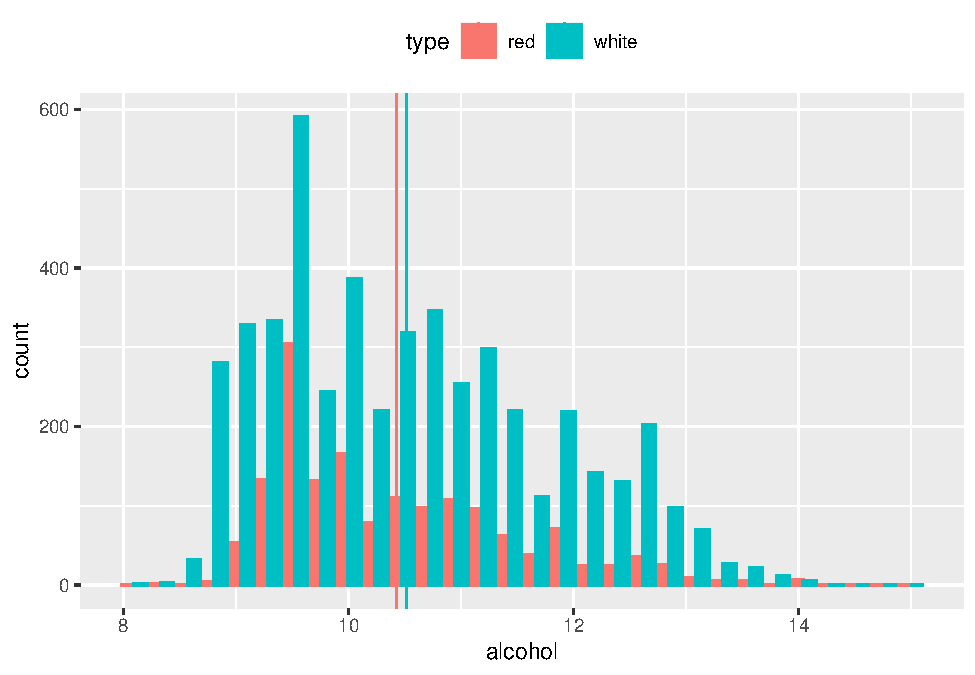
\includegraphics{FinalProject-Bright-Santoro_files/figure-latex/unnamed-chunk-3-1.pdf}

The table above shows the distribution of the alcohol variable for both red and white wines. We can see from the plot that alcohol does not appear to be normally distributed. The data points are primarily skewed to the left with a lower alcohol percentage. This makes sense as there are about three times as many white wine samples within our data set and white wine tends to have a lower alcohol percentage than red wine.

\begin{Shaded}
\begin{Highlighting}[]
\NormalTok{mu }\OtherTok{\textless{}{-}} \FunctionTok{ddply}\NormalTok{(wine, }\StringTok{"type"}\NormalTok{, summarise, }\AttributeTok{grp.mean=}\FunctionTok{mean}\NormalTok{(volatile.acidity))}

\NormalTok{g}\OtherTok{\textless{}{-}}\FunctionTok{ggplot}\NormalTok{(wine, }\FunctionTok{aes}\NormalTok{(}\AttributeTok{x=}\NormalTok{volatile.acidity, }\AttributeTok{fill=}\NormalTok{type, }\AttributeTok{color=}\NormalTok{type)) }\SpecialCharTok{+}
  \FunctionTok{geom\_histogram}\NormalTok{(}\AttributeTok{position=}\StringTok{"dodge"}\NormalTok{)}\SpecialCharTok{+}
  \FunctionTok{theme}\NormalTok{(}\AttributeTok{legend.position=}\StringTok{"top"}\NormalTok{) }\SpecialCharTok{+} 
  \FunctionTok{geom\_vline}\NormalTok{(}\AttributeTok{data=}\NormalTok{mu, }\FunctionTok{aes}\NormalTok{(}\AttributeTok{xintercept=}\NormalTok{grp.mean, }\AttributeTok{color=}\NormalTok{type))}\SpecialCharTok{+}
  \FunctionTok{theme}\NormalTok{(}\AttributeTok{legend.position=}\StringTok{"top"}\NormalTok{)}

\NormalTok{g}
\end{Highlighting}
\end{Shaded}

\begin{verbatim}
## `stat_bin()` using `bins = 30`. Pick better value with `binwidth`.
\end{verbatim}

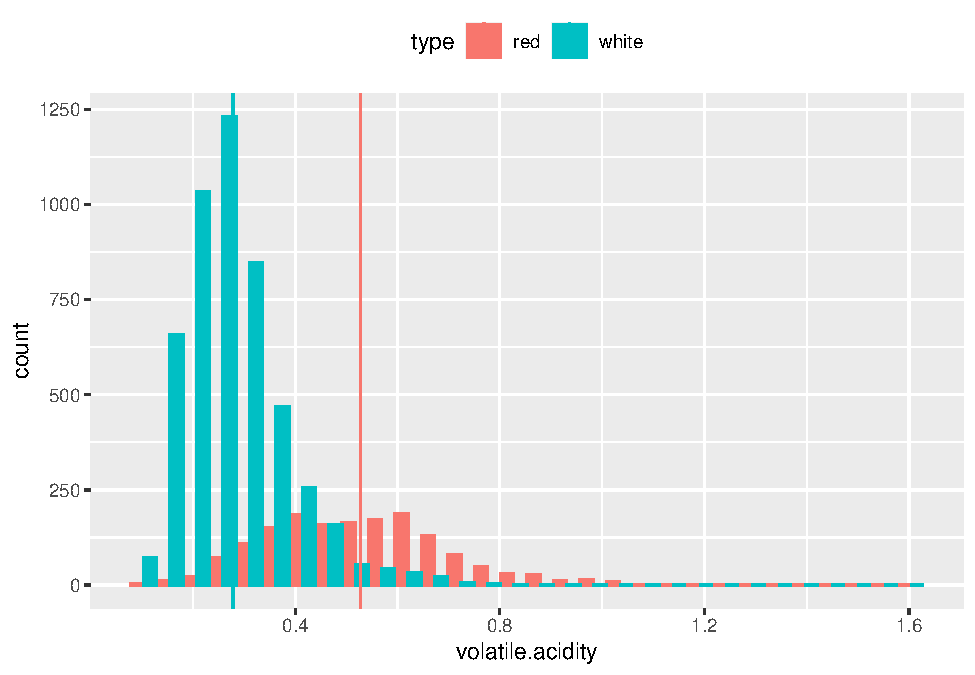
\includegraphics{FinalProject-Bright-Santoro_files/figure-latex/unnamed-chunk-4-1.pdf}

Volatile acidity is the amount of acetic acid in wine. Too high of a level of volatile acid can lead to an unpleasant, vinegar taste.

The distribution of volatile acidity measurements within red wine appeared to be fairly normally distributed, while the distribution in volatile acidity within white wine was skewed harshly to the right. However, both red and white wine samples had long tails which indicate there may be some outliers in the data set with higher levels of volatile acidity than normal.

\begin{Shaded}
\begin{Highlighting}[]
\NormalTok{mu }\OtherTok{\textless{}{-}} \FunctionTok{ddply}\NormalTok{(wine, }\StringTok{"type"}\NormalTok{, summarise, }\AttributeTok{grp.mean=}\FunctionTok{mean}\NormalTok{(quality))}

\NormalTok{g}\OtherTok{\textless{}{-}}\FunctionTok{ggplot}\NormalTok{(wine, }\FunctionTok{aes}\NormalTok{(}\AttributeTok{x=}\NormalTok{quality, }\AttributeTok{fill=}\NormalTok{type, }\AttributeTok{color=}\NormalTok{type)) }\SpecialCharTok{+}
  \FunctionTok{geom\_histogram}\NormalTok{(}\AttributeTok{position=}\StringTok{"dodge"}\NormalTok{)}\SpecialCharTok{+}
  \FunctionTok{theme}\NormalTok{(}\AttributeTok{legend.position=}\StringTok{"top"}\NormalTok{) }\SpecialCharTok{+} 
  \FunctionTok{geom\_vline}\NormalTok{(}\AttributeTok{data=}\NormalTok{mu, }\FunctionTok{aes}\NormalTok{(}\AttributeTok{xintercept=}\NormalTok{grp.mean, }\AttributeTok{color=}\NormalTok{type))}\SpecialCharTok{+}
  \FunctionTok{theme}\NormalTok{(}\AttributeTok{legend.position=}\StringTok{"top"}\NormalTok{)}

\NormalTok{g}
\end{Highlighting}
\end{Shaded}

\begin{verbatim}
## `stat_bin()` using `bins = 30`. Pick better value with `binwidth`.
\end{verbatim}

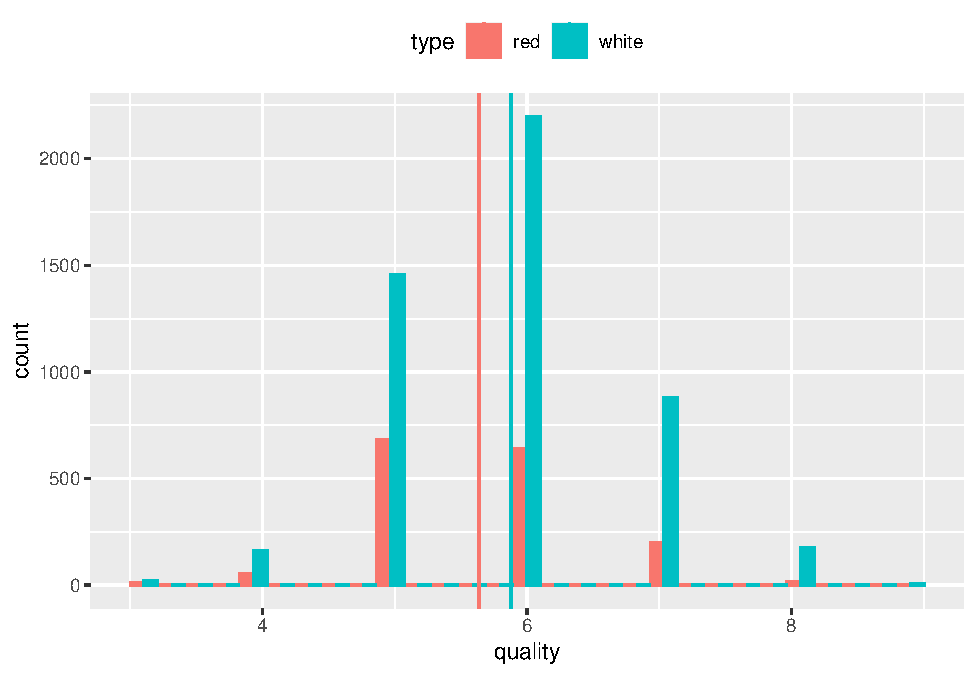
\includegraphics{FinalProject-Bright-Santoro_files/figure-latex/unnamed-chunk-5-1.pdf}

Finally, we plotted the quality, our outcome variable, of the wine samples. As you can see from the charts above both the red and white wine samples had a normal distribution of quality values. This is important to note as the tests we will be performing require or assume normally distributed outcome variable values.

\textbf{\emph{Bivariate Exploration}}

Bivariate exploration allows us to explore the relationship between two descriptive statistics in a dataset.

To better determine which variable relationships we should look more closely at, we ran a correlation analysis.

\begin{Shaded}
\begin{Highlighting}[]
\CommentTok{\# exclude the type of wine from the correlation variables }
\NormalTok{res }\OtherTok{\textless{}{-}} \FunctionTok{rcorr}\NormalTok{(}\FunctionTok{as.matrix}\NormalTok{(wine[,}\DecValTok{1}\SpecialCharTok{:}\DecValTok{12}\NormalTok{]))}
\NormalTok{corr }\OtherTok{\textless{}{-}} \FunctionTok{flattenCorrMatrix}\NormalTok{(res}\SpecialCharTok{$}\NormalTok{r, res}\SpecialCharTok{$}\NormalTok{P)}
\NormalTok{corr[}\FunctionTok{order}\NormalTok{(corr[,}\DecValTok{3}\NormalTok{],}\AttributeTok{decreasing=}\ConstantTok{TRUE}\NormalTok{),]}
\end{Highlighting}
\end{Shaded}

\begin{verbatim}
##                     row               column          cor            p
## 21  free.sulfur.dioxide total.sulfur.dioxide  0.720934081 0.000000e+00
## 25       residual.sugar              density  0.552516950 0.000000e+00
## 19       residual.sugar total.sulfur.dioxide  0.495481587 0.000000e+00
## 22        fixed.acidity              density  0.458909982 0.000000e+00
## 66              alcohol              quality  0.444318520 0.000000e+00
## 14       residual.sugar  free.sulfur.dioxide  0.402870640 0.000000e+00
## 41            chlorides            sulphates  0.395593307 0.000000e+00
## 8      volatile.acidity            chlorides  0.377124276 0.000000e+00
## 26            chlorides              density  0.362614656 0.000000e+00
## 2         fixed.acidity          citric.acid  0.324435725 0.000000e+00
## 37        fixed.acidity            sulphates  0.299567744 0.000000e+00
## 7         fixed.acidity            chlorides  0.298194772 0.000000e+00
## 23     volatile.acidity              density  0.271295648 0.000000e+00
## 30     volatile.acidity                   pH  0.261454403 0.000000e+00
## 44              density            sulphates  0.259478495 0.000000e+00
## 38     volatile.acidity            sulphates  0.225983680 0.000000e+00
## 1         fixed.acidity     volatile.acidity  0.219008256 0.000000e+00
## 18          citric.acid total.sulfur.dioxide  0.195241976 0.000000e+00
## 45                   pH            sulphates  0.192123407 0.000000e+00
## 6           citric.acid       residual.sugar  0.142451226 0.000000e+00
## 13          citric.acid  free.sulfur.dioxide  0.133125810 0.000000e+00
## 54                   pH              alcohol  0.121248467 0.000000e+00
## 24          citric.acid              density  0.096153929 7.993606e-15
## 58          citric.acid              quality  0.085531717 5.001777e-12
## 39          citric.acid            sulphates  0.056197300 5.830741e-06
## 61  free.sulfur.dioxide              quality  0.055463059 7.708445e-06
## 33            chlorides                   pH  0.044707980 3.124540e-04
## 9           citric.acid            chlorides  0.038998014 1.666635e-03
## 65            sulphates              quality  0.038485446 1.918079e-03
## 28 total.sulfur.dioxide              density  0.032394512 9.019631e-03
## 27  free.sulfur.dioxide              density  0.025716842 3.818871e-02
## 64                   pH              quality  0.019505704 1.159310e-01
## 36              density                   pH  0.011686081 3.462974e-01
## 55            sulphates              alcohol -0.003029195 8.071389e-01
## 48          citric.acid              alcohol -0.010493492 3.977326e-01
## 59       residual.sugar              quality -0.036980485 2.871025e-03
## 47     volatile.acidity              alcohol -0.037640386 2.409699e-03
## 62 total.sulfur.dioxide              quality -0.041385454 8.480397e-04
## 56        fixed.acidity              quality -0.076743208 5.874849e-10
## 46        fixed.acidity              alcohol -0.095451523 1.243450e-14
## 4         fixed.acidity       residual.sugar -0.111981281 0.000000e+00
## 10       residual.sugar            chlorides -0.128940500 0.000000e+00
## 34  free.sulfur.dioxide                   pH -0.145853896 0.000000e+00
## 51  free.sulfur.dioxide              alcohol -0.179838435 0.000000e+00
## 40       residual.sugar            sulphates -0.185927405 0.000000e+00
## 42  free.sulfur.dioxide            sulphates -0.188457249 0.000000e+00
## 15            chlorides  free.sulfur.dioxide -0.195044785 0.000000e+00
## 5      volatile.acidity       residual.sugar -0.196011174 0.000000e+00
## 60            chlorides              quality -0.200665500 0.000000e+00
## 35 total.sulfur.dioxide                   pH -0.238413103 0.000000e+00
## 29        fixed.acidity                   pH -0.252700468 0.000000e+00
## 50            chlorides              alcohol -0.256915580 0.000000e+00
## 57     volatile.acidity              quality -0.265699478 0.000000e+00
## 52 total.sulfur.dioxide              alcohol -0.265739639 0.000000e+00
## 32       residual.sugar                   pH -0.267319837 0.000000e+00
## 43 total.sulfur.dioxide            sulphates -0.275726820 0.000000e+00
## 20            chlorides total.sulfur.dioxide -0.279630447 0.000000e+00
## 11        fixed.acidity  free.sulfur.dioxide -0.282735428 0.000000e+00
## 63              density              quality -0.305857906 0.000000e+00
## 16        fixed.acidity total.sulfur.dioxide -0.329053901 0.000000e+00
## 31          citric.acid                   pH -0.329808191 0.000000e+00
## 12     volatile.acidity  free.sulfur.dioxide -0.352557306 0.000000e+00
## 49       residual.sugar              alcohol -0.359414771 0.000000e+00
## 3      volatile.acidity          citric.acid -0.377981317 0.000000e+00
## 17     volatile.acidity total.sulfur.dioxide -0.414476195 0.000000e+00
## 53              density              alcohol -0.686745421 0.000000e+00
\end{verbatim}

From the flatted correlation matrix above, we can see that the elements with the highest correlation are:
- Free Sulfur Dioxide and Total Sulfur Dioxide. This is intuitive as free sulfur dioxide is a subset of the total sulfur dioxide.
- Residual Sugar and Density. This also is intuitive as the fermentable sugars (residual sugar) can increase the density of wine.

\textbf{\emph{Visualize Correlations}}

\begin{Shaded}
\begin{Highlighting}[]
\CommentTok{\# Insignificant correlations are left blank}
\FunctionTok{corrplot}\NormalTok{(res}\SpecialCharTok{$}\NormalTok{r, }\AttributeTok{type=}\StringTok{"upper"}\NormalTok{, }\AttributeTok{order=}\StringTok{"hclust"}\NormalTok{, }
         \AttributeTok{p.mat =}\NormalTok{ res}\SpecialCharTok{$}\NormalTok{P, }\AttributeTok{sig.level =} \FloatTok{0.01}\NormalTok{, }\AttributeTok{insig =} \StringTok{"blank"}\NormalTok{)}
\end{Highlighting}
\end{Shaded}

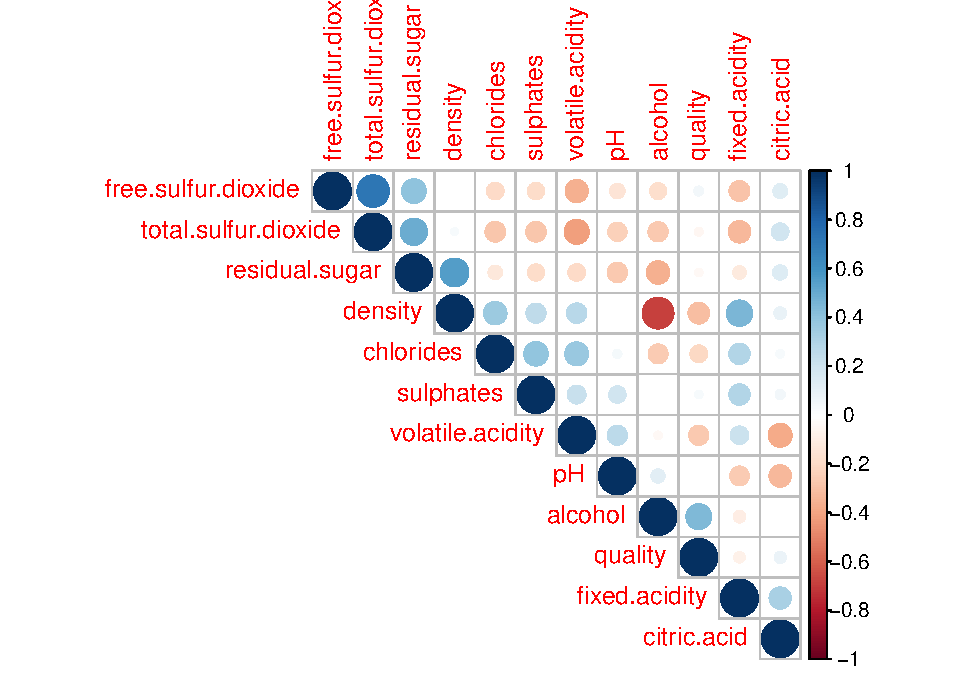
\includegraphics{FinalProject-Bright-Santoro_files/figure-latex/unnamed-chunk-7-1.pdf}

Based on the correlation matrix and the correlation plots it appears that there is a strong negative correlation between alcohol and density and a strong positive correlation between residual sugar and density. These are plotted below.

\begin{Shaded}
\begin{Highlighting}[]
\FunctionTok{ggplot}\NormalTok{(wine, }
       \FunctionTok{aes}\NormalTok{(}\AttributeTok{x =}\NormalTok{ alcohol, }
           \AttributeTok{y =}\NormalTok{ density, }
           \AttributeTok{color =}\NormalTok{ type)) }\SpecialCharTok{+}
  \FunctionTok{geom\_point}\NormalTok{(}\AttributeTok{size =} \DecValTok{3}\NormalTok{, }
             \AttributeTok{alpha =}\NormalTok{ .}\DecValTok{05}\NormalTok{) }\SpecialCharTok{+}
  \FunctionTok{labs}\NormalTok{(}\AttributeTok{title =} \StringTok{"Wine Composition by alcohol, density, and type"}\NormalTok{)}
\end{Highlighting}
\end{Shaded}

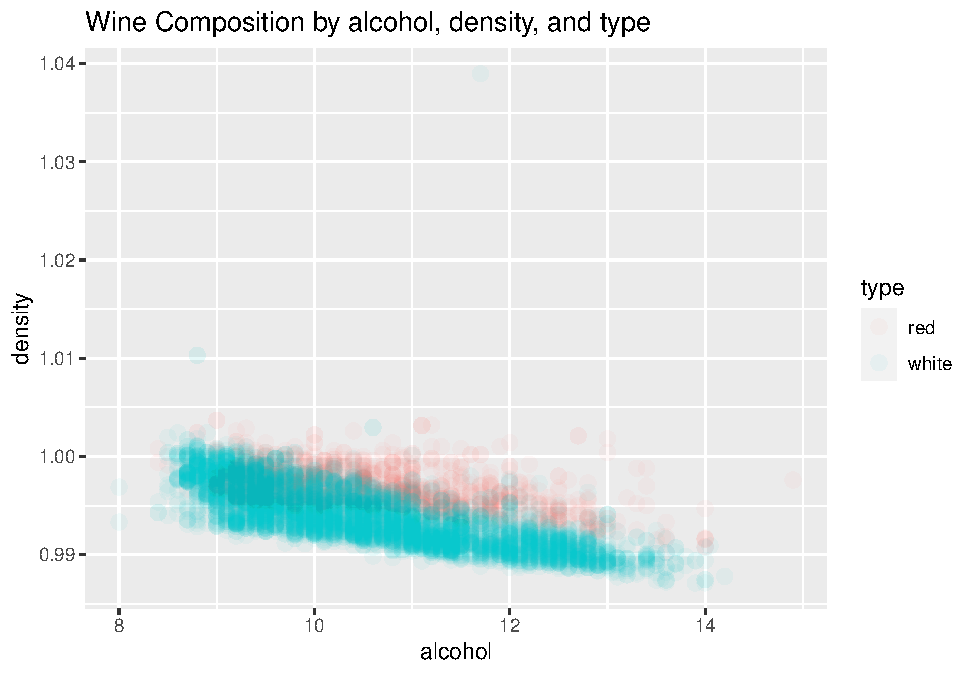
\includegraphics{FinalProject-Bright-Santoro_files/figure-latex/unnamed-chunk-8-1.pdf}

\begin{Shaded}
\begin{Highlighting}[]
\FunctionTok{ggplot}\NormalTok{(wine, }
       \FunctionTok{aes}\NormalTok{(}\AttributeTok{x =}\NormalTok{ residual.sugar, }
           \AttributeTok{y =}\NormalTok{ density, }
           \AttributeTok{color =}\NormalTok{ type)) }\SpecialCharTok{+}
  \FunctionTok{geom\_point}\NormalTok{(}\AttributeTok{size =} \DecValTok{3}\NormalTok{, }
             \AttributeTok{alpha =}\NormalTok{ .}\DecValTok{05}\NormalTok{) }\SpecialCharTok{+}
  \FunctionTok{labs}\NormalTok{(}\AttributeTok{title =} \StringTok{"Wine Composition by residual.sugar, density, and type"}\NormalTok{)}
\end{Highlighting}
\end{Shaded}

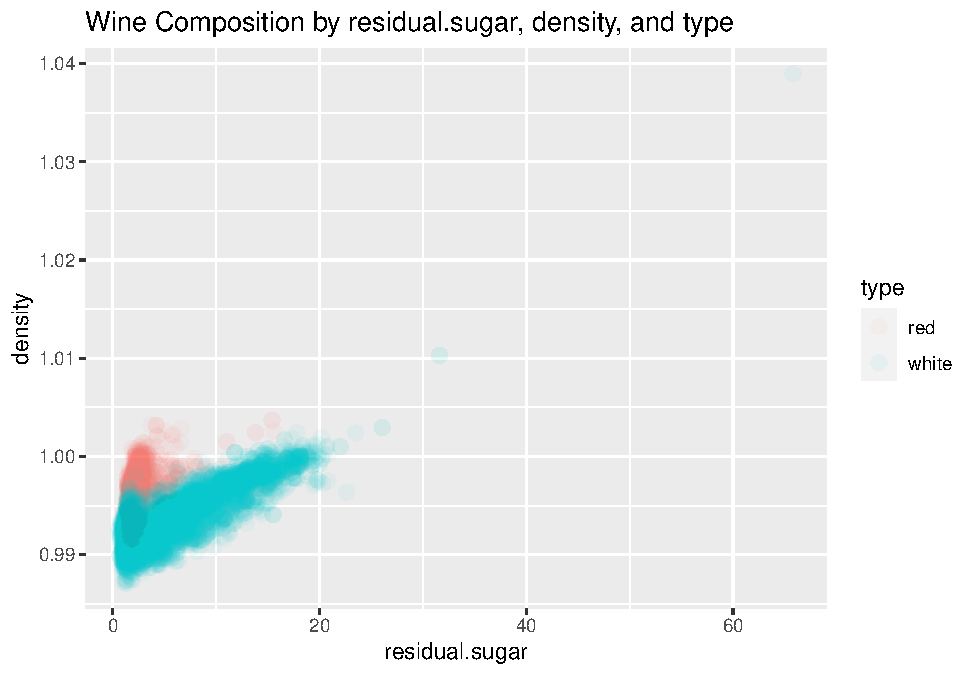
\includegraphics{FinalProject-Bright-Santoro_files/figure-latex/unnamed-chunk-9-1.pdf}

\hypertarget{data-cleaning-and-partitioning}{%
\chapter{Data Cleaning and Partitioning}\label{data-cleaning-and-partitioning}}

\hypertarget{data-normalization}{%
\section{Data Normalization}\label{data-normalization}}

Our dataset only contains input variables and outcome variable, so there was no need to remove descriptive data elements. However, we did normalize the input variables within the dataset to avoid any bias.

\begin{Shaded}
\begin{Highlighting}[]
\FunctionTok{set.seed}\NormalTok{(}\DecValTok{123}\NormalTok{)}

\CommentTok{\# do not include wine type in partitioned data.}
\NormalTok{wine }\OtherTok{\textless{}{-}}\NormalTok{wine[,}\DecValTok{1}\SpecialCharTok{:}\DecValTok{12}\NormalTok{]}
\CommentTok{\#Normalization}
\NormalTok{normalize }\OtherTok{\textless{}{-}} \ControlFlowTok{function}\NormalTok{(x) \{}
\FunctionTok{return}\NormalTok{ ((x }\SpecialCharTok{{-}} \FunctionTok{min}\NormalTok{(x)) }\SpecialCharTok{/}\NormalTok{ (}\FunctionTok{max}\NormalTok{(x) }\SpecialCharTok{{-}} \FunctionTok{min}\NormalTok{(x))) \}}

\CommentTok{\#De{-}Normalization}
\NormalTok{de.normalize }\OtherTok{\textless{}{-}} \ControlFlowTok{function}\NormalTok{(val)\{}
\NormalTok{  x }\OtherTok{\textless{}{-}}\NormalTok{ wine[,}\DecValTok{1}\SpecialCharTok{:}\DecValTok{12}\NormalTok{]}
  \FunctionTok{return}\NormalTok{ (val}\SpecialCharTok{*}\NormalTok{(}\FunctionTok{max}\NormalTok{(x) }\SpecialCharTok{{-}} \FunctionTok{min}\NormalTok{(x))}\SpecialCharTok{+}\FunctionTok{min}\NormalTok{(x))}
\NormalTok{\}}

\CommentTok{\#only normalize variables}
\NormalTok{wine.normal }\OtherTok{\textless{}{-}} \FunctionTok{as.data.frame}\NormalTok{(}\FunctionTok{lapply}\NormalTok{(wine[,}\DecValTok{1}\SpecialCharTok{:}\DecValTok{11}\NormalTok{], normalize))}

\CommentTok{\# add quality back }
\NormalTok{wine.normal}\SpecialCharTok{$}\NormalTok{quality }\OtherTok{=}\NormalTok{ wine}\SpecialCharTok{$}\NormalTok{quality}

\FunctionTok{head}\NormalTok{(wine.normal)}
\end{Highlighting}
\end{Shaded}

\begin{verbatim}
##   fixed.acidity volatile.acidity citric.acid residual.sugar chlorides
## 1     0.2975207        0.4133333  0.00000000     0.01993865 0.1112957
## 2     0.3305785        0.5333333  0.00000000     0.03067485 0.1478405
## 3     0.3305785        0.4533333  0.02409639     0.02607362 0.1378738
## 4     0.6115702        0.1333333  0.33734940     0.01993865 0.1096346
## 5     0.2975207        0.4133333  0.00000000     0.01993865 0.1112957
## 6     0.2975207        0.3866667  0.00000000     0.01840491 0.1096346
##   free.sulfur.dioxide total.sulfur.dioxide   density        pH sulphates
## 1          0.03472222           0.06451613 0.2060922 0.6124031 0.1910112
## 2          0.08333333           0.14055300 0.1868132 0.3720930 0.2584270
## 3          0.04861111           0.11059908 0.1906690 0.4186047 0.2415730
## 4          0.05555556           0.12442396 0.2099479 0.3410853 0.2022472
## 5          0.03472222           0.06451613 0.2060922 0.6124031 0.1910112
## 6          0.04166667           0.07834101 0.2060922 0.6124031 0.1910112
##     alcohol quality
## 1 0.2028986       5
## 2 0.2608696       5
## 3 0.2608696       5
## 4 0.2608696       6
## 5 0.2028986       5
## 6 0.2028986       5
\end{verbatim}

\hypertarget{data-partitioning}{%
\section{Data Partitioning}\label{data-partitioning}}

In order to determine whether our models are effective we must partition our dataset into a training and test set. We have decided to use \(70\%\) of our data for training and \(30\%\) for testing.

\begin{Shaded}
\begin{Highlighting}[]
\NormalTok{ind }\OtherTok{\textless{}{-}} \FunctionTok{sample}\NormalTok{(}\DecValTok{2}\NormalTok{, }\FunctionTok{nrow}\NormalTok{(wine.normal), }\AttributeTok{replace=}\ConstantTok{TRUE}\NormalTok{, }\AttributeTok{prob=}\FunctionTok{c}\NormalTok{(}\FloatTok{0.7}\NormalTok{, }\FloatTok{0.3}\NormalTok{))}

\NormalTok{train }\OtherTok{\textless{}{-}}\NormalTok{ wine.normal[ind}\SpecialCharTok{==}\DecValTok{1}\NormalTok{, ]}
\NormalTok{test }\OtherTok{\textless{}{-}}\NormalTok{ wine.normal[ind}\SpecialCharTok{==}\DecValTok{2}\NormalTok{,]}
\end{Highlighting}
\end{Shaded}

\hypertarget{comparing-results}{%
\section{Comparing Results}\label{comparing-results}}

We will be comparing accuracy of each of the methods so we will set up an accuracy data frame to compare the effectiveness of each of the methods.

\begin{Shaded}
\begin{Highlighting}[]
\NormalTok{accuracy }\OtherTok{\textless{}{-}} \FunctionTok{data.frame}\NormalTok{(}\AttributeTok{Accuracy=}\FunctionTok{c}\NormalTok{(}\FunctionTok{rep}\NormalTok{(}\ConstantTok{NA}\NormalTok{,}\AttributeTok{times=}\DecValTok{3}\NormalTok{)),}\AttributeTok{row.names =} \FunctionTok{c}\NormalTok{(}\StringTok{"K{-}Nearest"}\NormalTok{,}\StringTok{"Random Forest"}\NormalTok{,}\StringTok{"Regression"}\NormalTok{))}

\NormalTok{accuracy}
\end{Highlighting}
\end{Shaded}

\begin{verbatim}
##               Accuracy
## K-Nearest           NA
## Random Forest       NA
## Regression          NA
\end{verbatim}

\hypertarget{random-forest}{%
\chapter{Random Forest}\label{random-forest}}

The Random Forest modeling technique is a supervised machine learning algorithm that works by utilizing the outcome of multiple decision trees to make a prediction for a data point. It can be used to solve both classification and regression problems, however, for our analysis we utilized it to help solve our research question of classifying the quality of wine samples from 1-10. The algorithm can be tuned by a user by inputting a particular number of trees and variables to be tested at each split in the tree, in order to make it more precise.

"Each tree within the Random Forest is grown as follows:

\begin{enumerate}
\def\labelenumi{\arabic{enumi}.}
\tightlist
\item
  If the number of cases in the training set is N, sample N cases at random - but with replacement, from the original data. This sample will be the training set for growing the tree.
\item
  If there are M input variables, a number m\textless\textless M is specified such that at each node, m variables are selected at random out of the M and the best split on these m is used to split the node. The value of m is held constant during the forest growing.
\item
  Each tree is grown to the largest extent possible. There is no pruning." \citet{random_forests}
\end{enumerate}

\hypertarget{create-random-forest-model}{%
\section{Create Random Forest Model}\label{create-random-forest-model}}

We will start by running the randomForest function with our training dataset used to train the model.

\begin{Shaded}
\begin{Highlighting}[]
\FunctionTok{set.seed}\NormalTok{(}\DecValTok{444}\NormalTok{)}

\NormalTok{rf.train }\OtherTok{\textless{}{-}}\NormalTok{ train}
\NormalTok{rf.train}\SpecialCharTok{$}\NormalTok{quality }\OtherTok{\textless{}{-}}\FunctionTok{as.factor}\NormalTok{(rf.train}\SpecialCharTok{$}\NormalTok{quality)}

\NormalTok{rf.test }\OtherTok{\textless{}{-}}\NormalTok{ test}
\NormalTok{rf.test}\SpecialCharTok{$}\NormalTok{quality }\OtherTok{\textless{}{-}}\FunctionTok{as.factor}\NormalTok{(rf.test}\SpecialCharTok{$}\NormalTok{quality)}

\CommentTok{\# quality is a function of all other variables }
\NormalTok{rf }\OtherTok{\textless{}{-}} \FunctionTok{randomForest}\NormalTok{(quality}\SpecialCharTok{\textasciitilde{}}\NormalTok{., }\AttributeTok{data=}\NormalTok{rf.train)}
\FunctionTok{print}\NormalTok{(rf)}
\end{Highlighting}
\end{Shaded}

\begin{verbatim}
## 
## Call:
##  randomForest(formula = quality ~ ., data = rf.train) 
##                Type of random forest: classification
##                      Number of trees: 500
## No. of variables tried at each split: 3
## 
##         OOB estimate of  error rate: 32.91%
## Confusion matrix:
##   3  4    5    6   7  8 9 class.error
## 3 0  0   11    8   0  0 0   1.0000000
## 4 0 24   82   43   2  0 0   0.8410596
## 5 0  4 1086  421   7  0 0   0.2845850
## 6 0  1  335 1526 112  1 0   0.2273418
## 7 0  0   21  354 379  6 0   0.5013158
## 8 0  0    3   52  34 47 0   0.6544118
## 9 0  0    0    1   4  0 0   1.0000000
\end{verbatim}

The default number of trees was utilized to run our model (500) and the number of variables tried at each split in the tree was \(3\) variables.

The table above shows the confusion matrix for the random forest model created with the training dataset. The out-of-bag (OOB) error is shown to be \(32.91\%\). According to the class.error results, the model was most inaccurate when predicting wines with a quality of \(3\) or \(9\) with a \(100\%\) error rate. It was most accurate when predicting wines of value 6 with only a \(22\%\) error rate.

\hypertarget{predicition-and-confusion-matrix---training-data}{%
\section{Predicition and Confusion Matrix - Training Data}\label{predicition-and-confusion-matrix---training-data}}

The following code runs a prediction of the quality values for the training set using the random forest model created above.

As you can see, all 6 predictions in the predicted values vector are 100\% accurate. This makes sense as the random forest model was built using the training data, so it has already ``seen'' these values.

\begin{Shaded}
\begin{Highlighting}[]
\NormalTok{p1 }\OtherTok{\textless{}{-}} \FunctionTok{predict}\NormalTok{(rf, rf.train)}
\NormalTok{p1}\OtherTok{\textless{}{-}} \FunctionTok{droplevels}\NormalTok{(p1) }\CommentTok{\#drop any unused levels}
\FunctionTok{head}\NormalTok{(p1) }\CommentTok{\# predicted values}
\end{Highlighting}
\end{Shaded}

\begin{verbatim}
##  1  3  6  7  9 10 
##  5  5  5  5  7  5 
## Levels: 3 4 5 6 7 8 9
\end{verbatim}

\begin{Shaded}
\begin{Highlighting}[]
\FunctionTok{head}\NormalTok{(rf.train}\SpecialCharTok{$}\NormalTok{quality) }\CommentTok{\# actual values}
\end{Highlighting}
\end{Shaded}

\begin{verbatim}
## [1] 5 5 5 5 7 5
## Levels: 3 4 5 6 7 8 9
\end{verbatim}

\begin{Shaded}
\begin{Highlighting}[]
\CommentTok{\#install.packages(\textquotesingle{}caret\textquotesingle{}, dependencies = TRUE)}

\FunctionTok{confusionMatrix}\NormalTok{(p1, rf.train}\SpecialCharTok{$}\NormalTok{quality )}
\end{Highlighting}
\end{Shaded}

\begin{verbatim}
## Confusion Matrix and Statistics
## 
##           Reference
## Prediction    3    4    5    6    7    8    9
##          3   19    0    0    0    0    0    0
##          4    0  151    0    0    0    0    0
##          5    0    0 1518    0    0    0    0
##          6    0    0    0 1975    0    0    0
##          7    0    0    0    0  760    0    0
##          8    0    0    0    0    0  136    0
##          9    0    0    0    0    0    0    5
## 
## Overall Statistics
##                                      
##                Accuracy : 1          
##                  95% CI : (0.9992, 1)
##     No Information Rate : 0.4327     
##     P-Value [Acc > NIR] : < 2.2e-16  
##                                      
##                   Kappa : 1          
##                                      
##  Mcnemar's Test P-Value : NA         
## 
## Statistics by Class:
## 
##                      Class: 3 Class: 4 Class: 5 Class: 6 Class: 7 Class: 8
## Sensitivity          1.000000  1.00000   1.0000   1.0000   1.0000   1.0000
## Specificity          1.000000  1.00000   1.0000   1.0000   1.0000   1.0000
## Pos Pred Value       1.000000  1.00000   1.0000   1.0000   1.0000   1.0000
## Neg Pred Value       1.000000  1.00000   1.0000   1.0000   1.0000   1.0000
## Prevalence           0.004163  0.03309   0.3326   0.4327   0.1665   0.0298
## Detection Rate       0.004163  0.03309   0.3326   0.4327   0.1665   0.0298
## Detection Prevalence 0.004163  0.03309   0.3326   0.4327   0.1665   0.0298
## Balanced Accuracy    1.000000  1.00000   1.0000   1.0000   1.0000   1.0000
##                      Class: 9
## Sensitivity          1.000000
## Specificity          1.000000
## Pos Pred Value       1.000000
## Neg Pred Value       1.000000
## Prevalence           0.001096
## Detection Rate       0.001096
## Detection Prevalence 0.001096
## Balanced Accuracy    1.000000
\end{verbatim}

Using the confusion matrix function from the caret library, we can show the accuracy of our model when predicting the quality values for our training dataset. The accuracy is 100\% when utilizing the training dataset with the random forest model trained by the training dataset.

\hypertarget{predicition-and-confusion-matrix---test-data}{%
\section{Predicition and Confusion Matrix - Test Data}\label{predicition-and-confusion-matrix---test-data}}

The following code runs a prediction of the quality values for the test dataset using the random forest model created with our training dataset from above.

This model was able to predict 4 out of 6 of the first values accurately.

\begin{Shaded}
\begin{Highlighting}[]
\NormalTok{p2 }\OtherTok{\textless{}{-}} \FunctionTok{predict}\NormalTok{(rf, rf.test)}
\NormalTok{p2}\OtherTok{\textless{}{-}}\FunctionTok{droplevels}\NormalTok{(p2) }\CommentTok{\# drop unused levels}
\FunctionTok{head}\NormalTok{(p2) }\CommentTok{\# predicted values}
\end{Highlighting}
\end{Shaded}

\begin{verbatim}
##  2  4  5  8 11 16 
##  5  5  5  5  5  5 
## Levels: 3 4 5 6 7 8
\end{verbatim}

\begin{Shaded}
\begin{Highlighting}[]
\FunctionTok{head}\NormalTok{(rf.test}\SpecialCharTok{$}\NormalTok{quality) }\CommentTok{\# actual values}
\end{Highlighting}
\end{Shaded}

\begin{verbatim}
## [1] 5 6 5 7 5 5
## Levels: 3 4 5 6 7 8
\end{verbatim}

\begin{Shaded}
\begin{Highlighting}[]
\FunctionTok{confusionMatrix}\NormalTok{(p2, rf.test}\SpecialCharTok{$}\NormalTok{quality )}
\end{Highlighting}
\end{Shaded}

\begin{verbatim}
## Confusion Matrix and Statistics
## 
##           Reference
## Prediction   3   4   5   6   7   8
##          3   0   1   0   0   0   0
##          4   0   8   1   1   0   0
##          5   3  31 448 136   9   0
##          6   7  24 169 680 128  24
##          7   1   1   2  44 178  15
##          8   0   0   0   0   4  18
## 
## Overall Statistics
##                                           
##                Accuracy : 0.6891          
##                  95% CI : (0.6679, 0.7097)
##     No Information Rate : 0.4454          
##     P-Value [Acc > NIR] : < 2.2e-16       
##                                           
##                   Kappa : 0.512           
##                                           
##  Mcnemar's Test P-Value : NA              
## 
## Statistics by Class:
## 
##                       Class: 3 Class: 4 Class: 5 Class: 6 Class: 7 Class: 8
## Sensitivity          0.0000000 0.123077   0.7226   0.7898  0.55799 0.315789
## Specificity          0.9994797 0.998929   0.8637   0.6716  0.96097 0.997868
## Pos Pred Value       0.0000000 0.800000   0.7145   0.6589  0.73859 0.818182
## Neg Pred Value       0.9943064 0.970359   0.8683   0.7991  0.91667 0.979592
## Prevalence           0.0056906 0.033626   0.3207   0.4454  0.16503 0.029488
## Detection Rate       0.0000000 0.004139   0.2318   0.3518  0.09208 0.009312
## Detection Prevalence 0.0005173 0.005173   0.3244   0.5339  0.12468 0.011381
## Balanced Accuracy    0.4997399 0.561003   0.7931   0.7307  0.75948 0.656829
\end{verbatim}

Using the confusion matrix function from the caret library, we can show the accuracy of our model in predicting the quality values for our test dataset. The accuracy is roughly 69\% when utilizing the test dataset with the random forest model trained by the training dataset.

\hypertarget{tuning-our-model}{%
\section{Tuning our Model}\label{tuning-our-model}}

Now, that we have run our initial model, we can focus on fine tuning the random forest parameters in order to create a more accurate predictive model.

\hypertarget{plotting-the-error-rate}{%
\subsection{Plotting the Error Rate}\label{plotting-the-error-rate}}

Plotting the error rate to the number of trees can show us where our model has more or less the same level of effectiveness and we can choose a more accurate tree number.

\begin{Shaded}
\begin{Highlighting}[]
\FunctionTok{plot}\NormalTok{(rf)}
\end{Highlighting}
\end{Shaded}

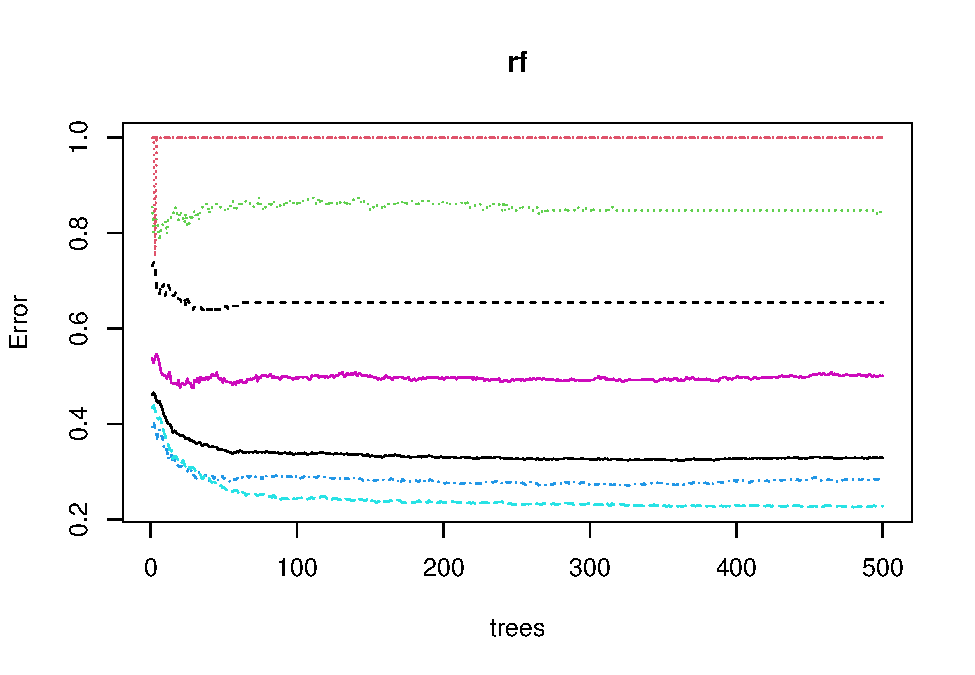
\includegraphics{FinalProject-Bright-Santoro_files/figure-latex/unnamed-chunk-18-1.pdf}
The model appears to have a drop off after about 300 trees and then is more or less constant, therefore, we can adjust our tree number in the model to be 300.

\hypertarget{tuning-mtry}{%
\subsection{Tuning mTry}\label{tuning-mtry}}

The mTry value reflects the number of variables tested at each node split. The tuneRF function can be used to determine what our mTry value should be.

\begin{Shaded}
\begin{Highlighting}[]
\FunctionTok{set.seed}\NormalTok{(}\DecValTok{2222}\NormalTok{)}

\NormalTok{t }\OtherTok{\textless{}{-}} \FunctionTok{tuneRF}\NormalTok{(rf.train[,}\SpecialCharTok{{-}}\DecValTok{12}\NormalTok{], rf.train[,}\DecValTok{12}\NormalTok{], }
       \AttributeTok{stepFactor =} \FloatTok{0.5}\NormalTok{, }
       \AttributeTok{plot=}\ConstantTok{TRUE}\NormalTok{,}
       \AttributeTok{ntreeTry =} \DecValTok{100}\NormalTok{,}
       \AttributeTok{trace=}\ConstantTok{TRUE}\NormalTok{,}
       \AttributeTok{improve=}\FloatTok{0.05}\NormalTok{)}
\end{Highlighting}
\end{Shaded}

\begin{verbatim}
## mtry = 3  OOB error = 33.26% 
## Searching left ...
## mtry = 6     OOB error = 34.36% 
## -0.03293808 0.05 
## Searching right ...
## mtry = 1     OOB error = 33.46% 
## -0.005928854 0.05
\end{verbatim}

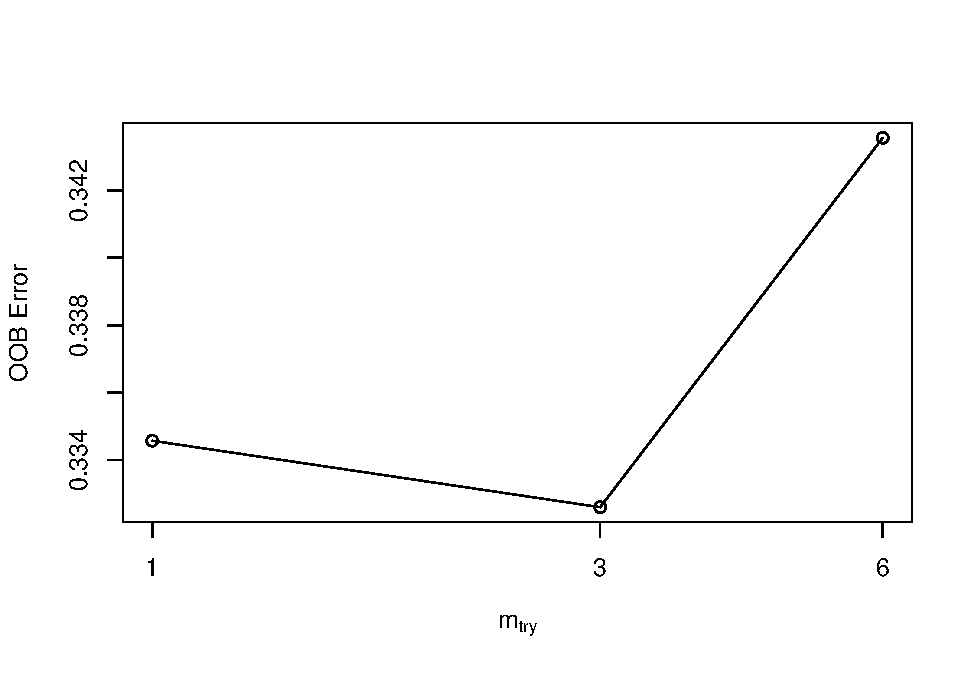
\includegraphics{FinalProject-Bright-Santoro_files/figure-latex/unnamed-chunk-19-1.pdf}
This output indicates that our model hits its lowest error rate when the mTry value is 3, so we can adjust our model to reflect this new value.

\hypertarget{recreate-our-random-forest-model}{%
\section{Recreate our Random Forest Model}\label{recreate-our-random-forest-model}}

The following code reruns our model utilizing the new tuning parameters found above.

\begin{Shaded}
\begin{Highlighting}[]
\FunctionTok{set.seed}\NormalTok{(}\DecValTok{444}\NormalTok{)}

\CommentTok{\# quality is a function of all other variables }
\NormalTok{rf }\OtherTok{\textless{}{-}} \FunctionTok{randomForest}\NormalTok{(quality}\SpecialCharTok{\textasciitilde{}}\NormalTok{., }\AttributeTok{data=}\NormalTok{rf.train,}
                   \AttributeTok{ntree=}\DecValTok{300}\NormalTok{,}
                   \AttributeTok{mTry=}\DecValTok{3}\NormalTok{, }
                   \AttributeTok{importance=}\ConstantTok{TRUE}\NormalTok{,}
                   \AttributeTok{proximity=}\ConstantTok{TRUE}\NormalTok{)}
\FunctionTok{print}\NormalTok{(rf)}
\end{Highlighting}
\end{Shaded}

\begin{verbatim}
## 
## Call:
##  randomForest(formula = quality ~ ., data = rf.train, ntree = 300,      mTry = 3, importance = TRUE, proximity = TRUE) 
##                Type of random forest: classification
##                      Number of trees: 300
## No. of variables tried at each split: 3
## 
##         OOB estimate of  error rate: 32.23%
## Confusion matrix:
##   3  4    5    6   7  8 9 class.error
## 3 0  1   10    8   0  0 0   1.0000000
## 4 0 21   85   45   0  0 0   0.8609272
## 5 0  5 1100  407   6  0 0   0.2753623
## 6 0  1  321 1537 115  1 0   0.2217722
## 7 0  0   22  343 388  7 0   0.4894737
## 8 0  0    4   55  30 47 0   0.6544118
## 9 0  0    0    1   4  0 0   1.0000000
\end{verbatim}

Our original OOB error rate was 32.91\% and utilizing our new tuned parameters, our OOB error rate was 32.23\%, so it was improved roughly 0.7\%.

\hypertarget{rerun-predicition-and-confusion-matrix---training-data}{%
\section{Rerun Predicition and Confusion Matrix - Training Data}\label{rerun-predicition-and-confusion-matrix---training-data}}

\begin{Shaded}
\begin{Highlighting}[]
\NormalTok{p1 }\OtherTok{\textless{}{-}} \FunctionTok{predict}\NormalTok{(rf, rf.train)}
\NormalTok{p1}\OtherTok{\textless{}{-}} \FunctionTok{droplevels}\NormalTok{(p1) }\CommentTok{\# drop any unused levels}
\FunctionTok{head}\NormalTok{(p1) }\CommentTok{\# predicted values}
\end{Highlighting}
\end{Shaded}

\begin{verbatim}
##  1  3  6  7  9 10 
##  5  5  5  5  7  5 
## Levels: 3 4 5 6 7 8 9
\end{verbatim}

\begin{Shaded}
\begin{Highlighting}[]
\FunctionTok{head}\NormalTok{(rf.train}\SpecialCharTok{$}\NormalTok{quality) }\CommentTok{\# actual values}
\end{Highlighting}
\end{Shaded}

\begin{verbatim}
## [1] 5 5 5 5 7 5
## Levels: 3 4 5 6 7 8 9
\end{verbatim}

\begin{Shaded}
\begin{Highlighting}[]
\FunctionTok{confusionMatrix}\NormalTok{(p1, rf.train}\SpecialCharTok{$}\NormalTok{quality )}
\end{Highlighting}
\end{Shaded}

\begin{verbatim}
## Confusion Matrix and Statistics
## 
##           Reference
## Prediction    3    4    5    6    7    8    9
##          3   19    0    0    0    0    0    0
##          4    0  151    0    0    0    0    0
##          5    0    0 1518    0    0    0    0
##          6    0    0    0 1975    0    0    0
##          7    0    0    0    0  760    0    0
##          8    0    0    0    0    0  136    0
##          9    0    0    0    0    0    0    5
## 
## Overall Statistics
##                                      
##                Accuracy : 1          
##                  95% CI : (0.9992, 1)
##     No Information Rate : 0.4327     
##     P-Value [Acc > NIR] : < 2.2e-16  
##                                      
##                   Kappa : 1          
##                                      
##  Mcnemar's Test P-Value : NA         
## 
## Statistics by Class:
## 
##                      Class: 3 Class: 4 Class: 5 Class: 6 Class: 7 Class: 8
## Sensitivity          1.000000  1.00000   1.0000   1.0000   1.0000   1.0000
## Specificity          1.000000  1.00000   1.0000   1.0000   1.0000   1.0000
## Pos Pred Value       1.000000  1.00000   1.0000   1.0000   1.0000   1.0000
## Neg Pred Value       1.000000  1.00000   1.0000   1.0000   1.0000   1.0000
## Prevalence           0.004163  0.03309   0.3326   0.4327   0.1665   0.0298
## Detection Rate       0.004163  0.03309   0.3326   0.4327   0.1665   0.0298
## Detection Prevalence 0.004163  0.03309   0.3326   0.4327   0.1665   0.0298
## Balanced Accuracy    1.000000  1.00000   1.0000   1.0000   1.0000   1.0000
##                      Class: 9
## Sensitivity          1.000000
## Specificity          1.000000
## Pos Pred Value       1.000000
## Neg Pred Value       1.000000
## Prevalence           0.001096
## Detection Rate       0.001096
## Detection Prevalence 0.001096
## Balanced Accuracy    1.000000
\end{verbatim}

Again, all of our predictions were 100\% accurate as the training data had already been ``seen'' by the model.

\hypertarget{rerun-predicition-and-confusion-matrix---test-data}{%
\section{Rerun Predicition and Confusion Matrix - Test Data}\label{rerun-predicition-and-confusion-matrix---test-data}}

\begin{Shaded}
\begin{Highlighting}[]
\NormalTok{p2 }\OtherTok{\textless{}{-}} \FunctionTok{predict}\NormalTok{(rf, rf.test)}
\NormalTok{p2 }\OtherTok{\textless{}{-}} \FunctionTok{droplevels}\NormalTok{(p2) }\CommentTok{\# drop any unuused levels }
\FunctionTok{head}\NormalTok{(p2) }\CommentTok{\# predicted values}
\end{Highlighting}
\end{Shaded}

\begin{verbatim}
##  2  4  5  8 11 16 
##  5  5  5  5  5  5 
## Levels: 3 4 5 6 7 8
\end{verbatim}

\begin{Shaded}
\begin{Highlighting}[]
\FunctionTok{head}\NormalTok{(rf.test}\SpecialCharTok{$}\NormalTok{quality) }\CommentTok{\# actual values}
\end{Highlighting}
\end{Shaded}

\begin{verbatim}
## [1] 5 6 5 7 5 5
## Levels: 3 4 5 6 7 8
\end{verbatim}

\begin{Shaded}
\begin{Highlighting}[]
\FunctionTok{confusionMatrix}\NormalTok{(p2, rf.test}\SpecialCharTok{$}\NormalTok{quality )}
\end{Highlighting}
\end{Shaded}

\begin{verbatim}
## Confusion Matrix and Statistics
## 
##           Reference
## Prediction   3   4   5   6   7   8
##          3   0   1   0   0   0   0
##          4   0   8   1   2   0   0
##          5   3  32 447 139  10   0
##          6   7  23 170 675 130  25
##          7   1   1   2  45 175  14
##          8   0   0   0   0   4  18
## 
## Overall Statistics
##                                           
##                Accuracy : 0.6844          
##                  95% CI : (0.6632, 0.7051)
##     No Information Rate : 0.4454          
##     P-Value [Acc > NIR] : < 2.2e-16       
##                                           
##                   Kappa : 0.5047          
##                                           
##  Mcnemar's Test P-Value : NA              
## 
## Statistics by Class:
## 
##                       Class: 3 Class: 4 Class: 5 Class: 6 Class: 7 Class: 8
## Sensitivity          0.0000000 0.123077   0.7210   0.7840  0.54859 0.315789
## Specificity          0.9994797 0.998394   0.8599   0.6688  0.96097 0.997868
## Pos Pred Value       0.0000000 0.727273   0.7084   0.6553  0.73529 0.818182
## Neg Pred Value       0.9943064 0.970343   0.8671   0.7940  0.91504 0.979592
## Prevalence           0.0056906 0.033626   0.3207   0.4454  0.16503 0.029488
## Detection Rate       0.0000000 0.004139   0.2312   0.3492  0.09053 0.009312
## Detection Prevalence 0.0005173 0.005691   0.3264   0.5329  0.12312 0.011381
## Balanced Accuracy    0.4997399 0.560735   0.7904   0.7264  0.75478 0.656829
\end{verbatim}

The accuracy is roughly \(68.24\%\) when utilizing the test dataset with the new random forest model. This is a \(0.7\%\) improvement from the previous results of \(68.91\%\).

\hypertarget{variable-importance}{%
\section{Variable Importance}\label{variable-importance}}

We are able to see the variables that had the highest level of importance in our model by running the varImpPlot function.

\begin{Shaded}
\begin{Highlighting}[]
\FunctionTok{varImpPlot}\NormalTok{(rf, }
           \AttributeTok{main=}\StringTok{"Variable Importance"}\NormalTok{)}
\end{Highlighting}
\end{Shaded}

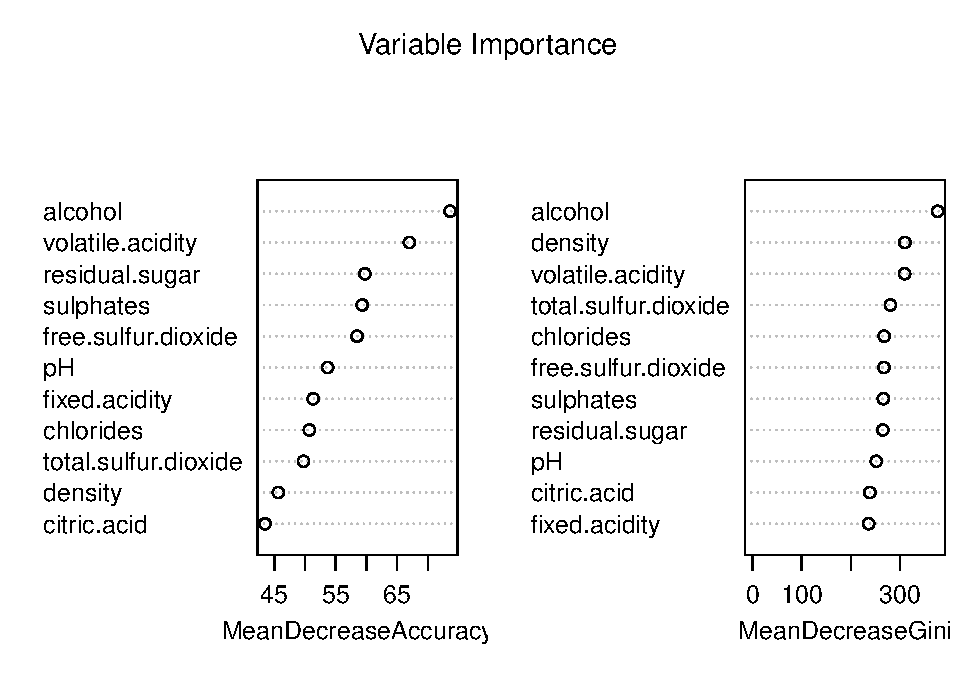
\includegraphics{FinalProject-Bright-Santoro_files/figure-latex/unnamed-chunk-25-1.pdf}
This tells us that alcohol has the greatest importance in our model. Removing this variable would result in a 75\% mean decrease in accuracy.

\hypertarget{accuracy}{%
\section{Accuracy}\label{accuracy}}

In the code below we are adding the percentage accuracy to the accuracy dataframe for later model comparison.

\begin{Shaded}
\begin{Highlighting}[]
\NormalTok{accuracy[}\DecValTok{2}\NormalTok{,}\DecValTok{1}\NormalTok{] }\OtherTok{\textless{}{-}} \FunctionTok{confusionMatrix}\NormalTok{(p2, rf.test}\SpecialCharTok{$}\NormalTok{quality )[[}\StringTok{"overall"}\NormalTok{]][[}\StringTok{"Accuracy"}\NormalTok{]]}
\end{Highlighting}
\end{Shaded}

\hypertarget{k-nearest-neighbor}{%
\chapter{K-Nearest Neighbor}\label{k-nearest-neighbor}}

K-Nearest Neighbor (KNN) is another supervised machine learning algorithm that can classify a new data point by comparing the data points variable or factors to the variables or factors of its ``nearest neighbors''. KNN is also able to solve both classification and regression problems, however, we utilized it to solve our research question of classifying the quality of wine samples from 1-10. The algorithm for KNN determines a data points ``nearest neighbors'' by computing the Euclidean distance between the points. Then, similarly to Random Forest, KNN uses the consensus of those neighbors to predict the outcome variable for the new data point. \citet{knn}

\hypertarget{data-partitioning-1}{%
\section{Data Partitioning}\label{data-partitioning-1}}

Our data has already been randomly partitioned into training and test data sets, however, the KNN algorithm we are utilizing within the caret library requires that we make our quality variables a ``factor'' data type.

\begin{Shaded}
\begin{Highlighting}[]
\FunctionTok{set.seed}\NormalTok{(}\DecValTok{444}\NormalTok{)}

\NormalTok{knn.train }\OtherTok{\textless{}{-}}\NormalTok{ train}
\NormalTok{knn.train}\SpecialCharTok{$}\NormalTok{quality }\OtherTok{\textless{}{-}}\FunctionTok{as.factor}\NormalTok{(knn.train}\SpecialCharTok{$}\NormalTok{quality)}

\NormalTok{knn.test }\OtherTok{\textless{}{-}}\NormalTok{ test}
\NormalTok{knn.test}\SpecialCharTok{$}\NormalTok{quality }\OtherTok{\textless{}{-}}\FunctionTok{as.factor}\NormalTok{(knn.test}\SpecialCharTok{$}\NormalTok{quality)}

\FunctionTok{str}\NormalTok{(knn.test)}
\end{Highlighting}
\end{Shaded}

\begin{verbatim}
## 'data.frame':    1933 obs. of  12 variables:
##  $ fixed.acidity       : num  0.331 0.612 0.298 0.289 0.24 ...
##  $ volatile.acidity    : num  0.533 0.133 0.413 0.38 0.333 ...
##  $ citric.acid         : num  0 0.3373 0 0 0.0482 ...
##  $ residual.sugar      : num  0.0307 0.0199 0.0199 0.0092 0.0184 ...
##  $ chlorides           : num  0.148 0.11 0.111 0.093 0.146 ...
##  $ free.sulfur.dioxide : num  0.0833 0.0556 0.0347 0.0486 0.0486 ...
##  $ total.sulfur.dioxide: num  0.1406 0.1244 0.0645 0.0346 0.1359 ...
##  $ density             : num  0.187 0.21 0.206 0.144 0.169 ...
##  $ pH                  : num  0.372 0.341 0.612 0.519 0.434 ...
##  $ sulphates           : num  0.258 0.202 0.191 0.14 0.18 ...
##  $ alcohol             : num  0.261 0.261 0.203 0.29 0.174 ...
##  $ quality             : Factor w/ 6 levels "3","4","5","6",..: 3 4 3 5 3 3 4 4 3 3 ...
\end{verbatim}

\begin{Shaded}
\begin{Highlighting}[]
\FunctionTok{str}\NormalTok{(knn.train)}
\end{Highlighting}
\end{Shaded}

\begin{verbatim}
## 'data.frame':    4564 obs. of  12 variables:
##  $ fixed.acidity       : num  0.298 0.331 0.298 0.339 0.331 ...
##  $ volatile.acidity    : num  0.413 0.453 0.387 0.347 0.333 ...
##  $ citric.acid         : num  0 0.0241 0 0.0361 0.012 ...
##  $ residual.sugar      : num  0.0199 0.0261 0.0184 0.0153 0.0215 ...
##  $ chlorides           : num  0.1113 0.1379 0.1096 0.0997 0.1063 ...
##  $ free.sulfur.dioxide : num  0.0347 0.0486 0.0417 0.0486 0.0278 ...
##  $ total.sulfur.dioxide: num  0.0645 0.1106 0.0783 0.1221 0.0276 ...
##  $ density             : num  0.206 0.191 0.206 0.179 0.187 ...
##  $ pH                  : num  0.612 0.419 0.612 0.45 0.496 ...
##  $ sulphates           : num  0.191 0.242 0.191 0.135 0.197 ...
##  $ alcohol             : num  0.203 0.261 0.203 0.203 0.217 ...
##  $ quality             : Factor w/ 7 levels "3","4","5","6",..: 3 3 3 3 5 3 3 3 3 3 ...
\end{verbatim}

Because our data was randomly partitioned you can see there are 7 levels within quality factor in the train data, while there are only 6 levels within the quality factor in the test data. This will have to be managed later using the ``droplevels'' function, to find the accuracy using the confusionmatrix.

\hypertarget{determine-the-k-value}{%
\section{Determine the k-value}\label{determine-the-k-value}}

The k-value in the KNN algorithm determines how many of the nearest neighbors we will use to calculate our predicted quality. There are many different methods for computing the value of K, however, caret provides a built in library function ``train'' to help determine what the k-value we should utilize is.

``train'' utilizes k-fold cross validation to determine the accuracy of each k-value value. For our model, we used the repeated cross-validation method which indicates using cross-validation and repeating it a number of times to ensure accuracy. For our parameters, we chose to repeat 5 times and left the default number of folds to 10, as that has been previously found to result in a low-bias model.

Within the train function, we define the method for training our model to be ``knn'' for k-nearest neighbor and our tune length to be 40. The tuneLength parameter tells the algorithm to try 40 different values of k.

\begin{Shaded}
\begin{Highlighting}[]
\FunctionTok{set.seed}\NormalTok{(}\DecValTok{400}\NormalTok{)}
\NormalTok{tc }\OtherTok{\textless{}{-}} \FunctionTok{trainControl}\NormalTok{(}\AttributeTok{method=}\StringTok{"repeatedcv"}\NormalTok{,}\AttributeTok{repeats =} \DecValTok{5}\NormalTok{) }\CommentTok{\#,classProbs=TRUE,summaryFunction = twoClassSummary)}
\NormalTok{k.value }\OtherTok{\textless{}{-}} \FunctionTok{train}\NormalTok{(quality }\SpecialCharTok{\textasciitilde{}}\NormalTok{ ., }\AttributeTok{data =}\NormalTok{ knn.train, }\AttributeTok{method =} \StringTok{"knn"}\NormalTok{, }\AttributeTok{trControl =}\NormalTok{ tc, }\AttributeTok{tuneLength=}\DecValTok{40}\NormalTok{)}

\NormalTok{k.value}
\end{Highlighting}
\end{Shaded}

\begin{verbatim}
## k-Nearest Neighbors 
## 
## 4564 samples
##   11 predictor
##    7 classes: '3', '4', '5', '6', '7', '8', '9' 
## 
## No pre-processing
## Resampling: Cross-Validated (10 fold, repeated 5 times) 
## Summary of sample sizes: 4108, 4108, 4106, 4108, 4108, 4109, ... 
## Resampling results across tuning parameters:
## 
##   k   Accuracy   Kappa    
##    5  0.5321658  0.2858505
##    7  0.5389564  0.2902098
##    9  0.5389154  0.2868803
##   11  0.5335706  0.2749516
##   13  0.5314191  0.2693456
##   15  0.5371607  0.2765031
##   17  0.5348392  0.2710070
##   19  0.5356741  0.2702315
##   21  0.5383901  0.2736512
##   23  0.5388281  0.2735700
##   25  0.5416298  0.2764623
##   27  0.5418483  0.2759878
##   29  0.5397452  0.2716491
##   31  0.5434266  0.2766398
##   33  0.5410587  0.2723851
##   35  0.5418060  0.2724562
##   37  0.5423318  0.2729050
##   39  0.5420259  0.2713667
##   41  0.5432096  0.2732347
##   43  0.5431208  0.2726629
##   45  0.5408835  0.2686819
##   47  0.5414967  0.2691622
##   49  0.5410156  0.2676621
##   51  0.5408815  0.2668637
##   53  0.5395240  0.2638237
##   55  0.5391279  0.2630925
##   57  0.5389955  0.2621340
##   59  0.5379898  0.2603583
##   61  0.5393910  0.2621689
##   63  0.5371996  0.2589008
##   65  0.5373285  0.2588102
##   67  0.5378552  0.2590151
##   69  0.5373315  0.2577817
##   71  0.5372894  0.2572961
##   73  0.5364118  0.2556921
##   75  0.5384289  0.2584713
##   77  0.5382081  0.2577366
##   79  0.5377703  0.2569147
##   81  0.5377717  0.2563957
##   83  0.5358855  0.2530376
## 
## Accuracy was used to select the optimal model using the largest value.
## The final value used for the model was k = 31.
\end{verbatim}

The plot below shows the accuracy of the repeated cross-validation models to the k-values from train. We can see that the highest level of accuracy was hit at k=37 and then appears to decrease in accuracy as k increases.

\begin{Shaded}
\begin{Highlighting}[]
\FunctionTok{plot}\NormalTok{(k.value)}
\end{Highlighting}
\end{Shaded}

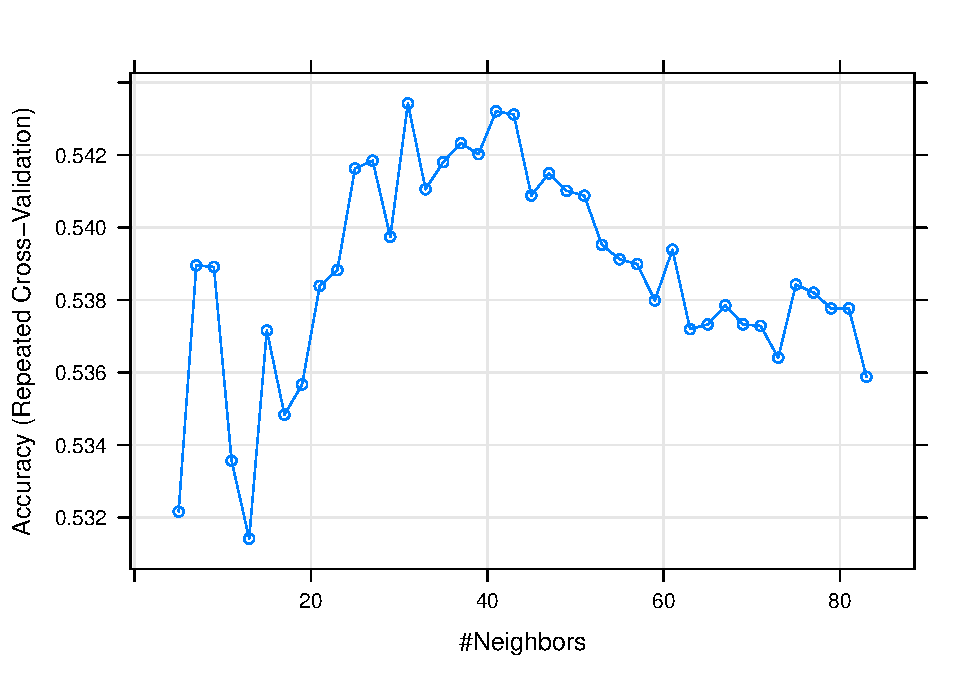
\includegraphics{FinalProject-Bright-Santoro_files/figure-latex/unnamed-chunk-29-1.pdf}

\hypertarget{knn-prediction}{%
\section{KNN Prediction}\label{knn-prediction}}

Now that we have our k-value and knn model trained, we can use it to predict our test values. In this portion of code, we will also account for the missing level from the quality factor that we found earlier, so that we can compute our confusion matrix.

\begin{Shaded}
\begin{Highlighting}[]
\NormalTok{knnPredict }\OtherTok{\textless{}{-}} \FunctionTok{predict}\NormalTok{(k.value,}\AttributeTok{newdata =}\NormalTok{ knn.test )}
\NormalTok{knnPredict}\FloatTok{.2}\OtherTok{\textless{}{-}}\FunctionTok{droplevels}\NormalTok{(knnPredict)}

\CommentTok{\#Get the confusion matrix to see accuracy value and other parameter values}
\FunctionTok{confusionMatrix}\NormalTok{(knnPredict}\FloatTok{.2}\NormalTok{, knn.test}\SpecialCharTok{$}\NormalTok{quality )}
\end{Highlighting}
\end{Shaded}

\begin{verbatim}
## Warning in levels(reference) != levels(data): longer object length is not a
## multiple of shorter object length
\end{verbatim}

\begin{verbatim}
## Warning in confusionMatrix.default(knnPredict.2, knn.test$quality): Levels are
## not in the same order for reference and data. Refactoring data to match.
\end{verbatim}

\begin{verbatim}
## Confusion Matrix and Statistics
## 
##           Reference
## Prediction   3   4   5   6   7   8
##          3   0   0   0   0   0   0
##          4   0   0   0   0   0   0
##          5   5  40 380 197  10   0
##          6   5  23 226 587 188  27
##          7   1   2  14  76 121  30
##          8   0   0   0   1   0   0
## 
## Overall Statistics
##                                           
##                Accuracy : 0.5629          
##                  95% CI : (0.5404, 0.5851)
##     No Information Rate : 0.4454          
##     P-Value [Acc > NIR] : < 2.2e-16       
##                                           
##                   Kappa : 0.3072          
##                                           
##  Mcnemar's Test P-Value : NA              
## 
## Statistics by Class:
## 
##                      Class: 3 Class: 4 Class: 5 Class: 6 Class: 7  Class: 8
## Sensitivity          0.000000  0.00000   0.6129   0.6818   0.3793 0.0000000
## Specificity          1.000000  1.00000   0.8081   0.5625   0.9238 0.9994670
## Pos Pred Value            NaN      NaN   0.6013   0.5559   0.4959 0.0000000
## Neg Pred Value       0.994309  0.96637   0.8155   0.6876   0.8828 0.9704969
## Prevalence           0.005691  0.03363   0.3207   0.4454   0.1650 0.0294878
## Detection Rate       0.000000  0.00000   0.1966   0.3037   0.0626 0.0000000
## Detection Prevalence 0.000000  0.00000   0.3270   0.5463   0.1262 0.0005173
## Balanced Accuracy    0.500000  0.50000   0.7105   0.6221   0.6516 0.4997335
\end{verbatim}

Our model was found to be about 56.75\% accurate in predicting quality measures for our wine samples.

\hypertarget{accuracy-1}{%
\section{Accuracy}\label{accuracy-1}}

In the code below we are adding the percentage accuracy to the accuracy dataframe for later model comparison.

\begin{Shaded}
\begin{Highlighting}[]
\NormalTok{accuracy[}\DecValTok{1}\NormalTok{,}\DecValTok{1}\NormalTok{] }\OtherTok{\textless{}{-}} \FunctionTok{confusionMatrix}\NormalTok{(knnPredict}\FloatTok{.2}\NormalTok{, knn.test}\SpecialCharTok{$}\NormalTok{quality )[[}\StringTok{"overall"}\NormalTok{]][[}\StringTok{"Accuracy"}\NormalTok{]]}
\end{Highlighting}
\end{Shaded}

\begin{verbatim}
## Warning in levels(reference) != levels(data): longer object length is not a
## multiple of shorter object length
\end{verbatim}

\begin{verbatim}
## Warning in confusionMatrix.default(knnPredict.2, knn.test$quality): Levels are
## not in the same order for reference and data. Refactoring data to match.
\end{verbatim}

\hypertarget{lasso-regression}{%
\chapter{Lasso Regression}\label{lasso-regression}}

\hypertarget{linear-regression}{%
\section{Linear Regression}\label{linear-regression}}

\hypertarget{what-is-it}{%
\subsection{What is it?}\label{what-is-it}}

The simplest form of regression is linear regression, which assumes that the predictors have a linear relationship with the target variable. \citet{regression_r}\\

\hypertarget{assumptions}{%
\subsection{Assumptions}\label{assumptions}}

Input is assumed to have a Normal distribution and are not correlated with each other.

We saw in the Descriptive Stats section that visually this factor had a strong correlation with quality.

With these assumptions being true we can model quality with the following equation. \citet{elastic_net}

\[ q = a_1x_1 + a_2x_2 + a_3x_3 + \dots + a_2nx_n + b + \epsilon\]
Where \(a_1, a_2, \dots, a_n\) are coefficients from the model. \(x_1, x_2, \dots, x_n\) are the input variables to the model. \(b\) is a factor of the model representing the y-intercept and \(q\) is equal to the quality output. Finally, \(\epsilon\) is the error.
The method that we use to optimize this model is Ordinary Least Squares (OLS).

\hypertarget{single-variable}{%
\subsection{Single Variable}\label{single-variable}}

In the code-block below we output the summary of just the measurement alcohol into the linear model.

\begin{Shaded}
\begin{Highlighting}[]
\NormalTok{lr}\FloatTok{.1} \OtherTok{\textless{}{-}} \FunctionTok{lm}\NormalTok{(quality}\SpecialCharTok{\textasciitilde{}}\NormalTok{alcohol, }\AttributeTok{data =}\NormalTok{ train)}
\FunctionTok{summary}\NormalTok{(lr}\FloatTok{.1}\NormalTok{)}
\end{Highlighting}
\end{Shaded}

\begin{verbatim}
## 
## Call:
## lm(formula = quality ~ alcohol, data = train)
## 
## Residuals:
##     Min      1Q  Median      3Q     Max 
## -3.4417 -0.5005 -0.0522  0.4995  3.2074 
## 
## Coefficients:
##             Estimate Std. Error t value Pr(>|t|)    
## (Intercept)  5.01358    0.02706  185.29   <2e-16 ***
## alcohol      2.23962    0.06800   32.94   <2e-16 ***
## ---
## Signif. codes:  0 '***' 0.001 '**' 0.01 '*' 0.05 '.' 0.1 ' ' 1
## 
## Residual standard error: 0.7863 on 4562 degrees of freedom
## Multiple R-squared:  0.1921, Adjusted R-squared:  0.1919 
## F-statistic:  1085 on 1 and 4562 DF,  p-value: < 2.2e-16
\end{verbatim}

Focusing on the p-value above we can tell that it is unlikely that by chance we will observe a relationship between alcohol and quality. Which fits our standard threshold of \(5\%\).
We will use the Root Mean Square Error (RMSE) to compare the results of each of the models. \citet{RMSE} The Root Mean Square Error (RMSE) is the standard deviation of the residuals (prediction errors). Residuals are a measure of how far from the regression line data points are; RMSE is a measure of how spread out these residuals are. In other words, it tells you how concentrated the data is around the line of best fit. We are looking for a value very close to zero here as the formula is as follows:

\[RMSE = \sqrt{\frac{\sum_{i=1}^{N}(predicted_i - actual_i)^2}{N}}\]

\begin{Shaded}
\begin{Highlighting}[]
\NormalTok{p}\FloatTok{.1} \OtherTok{\textless{}{-}} \FunctionTok{predict}\NormalTok{(lr}\FloatTok{.1}\NormalTok{, }\AttributeTok{newdata =}\NormalTok{ test)}
\NormalTok{RMSE}\FloatTok{.1} \OtherTok{\textless{}{-}} \FunctionTok{RMSE}\NormalTok{(p}\FloatTok{.1}\NormalTok{,test}\SpecialCharTok{$}\NormalTok{quality)}
\NormalTok{RMSE}\FloatTok{.1}
\end{Highlighting}
\end{Shaded}

\begin{verbatim}
## [1] 0.77316
\end{verbatim}

Since we will be comparing results to other discrete statistical methods we now calculate an accuracy measure.

\begin{Shaded}
\begin{Highlighting}[]
\NormalTok{rp}\FloatTok{.1}\OtherTok{\textless{}{-}}\FunctionTok{round}\NormalTok{(p}\FloatTok{.1}\NormalTok{)}
\NormalTok{acc}\FloatTok{.1} \OtherTok{\textless{}{-}} \FunctionTok{mean}\NormalTok{(rp}\FloatTok{.1}\SpecialCharTok{==}\NormalTok{test}\SpecialCharTok{$}\NormalTok{quality)}
\end{Highlighting}
\end{Shaded}

\hypertarget{multiple-variables}{%
\subsection{Multiple Variables}\label{multiple-variables}}

In the code block below we will input all of the variables and examine the output.

\begin{Shaded}
\begin{Highlighting}[]
\NormalTok{lr}\FloatTok{.2} \OtherTok{\textless{}{-}} \FunctionTok{lm}\NormalTok{(quality}\SpecialCharTok{\textasciitilde{}}\NormalTok{., }\AttributeTok{data =}\NormalTok{ train)}
\FunctionTok{summary}\NormalTok{(lr}\FloatTok{.2}\NormalTok{)}
\end{Highlighting}
\end{Shaded}

\begin{verbatim}
## 
## Call:
## lm(formula = quality ~ ., data = train)
## 
## Residuals:
##     Min      1Q  Median      3Q     Max 
## -3.6204 -0.4638 -0.0460  0.4627  2.9628 
## 
## Coefficients:
##                      Estimate Std. Error t value Pr(>|t|)    
## (Intercept)           5.21981    0.09286  56.213  < 2e-16 ***
## fixed.acidity         0.93217    0.22387   4.164 3.19e-05 ***
## volatile.acidity     -2.06695    0.13890 -14.880  < 2e-16 ***
## citric.acid          -0.29888    0.15704  -1.903   0.0571 .  
## residual.sugar        3.12413    0.39967   7.817 6.68e-15 ***
## chlorides            -0.37223    0.22612  -1.646   0.0998 .  
## free.sulfur.dioxide   1.58600    0.25778   6.153 8.28e-10 ***
## total.sulfur.dioxide -1.11244    0.14508  -7.668 2.12e-14 ***
## density              -3.12231    0.73831  -4.229 2.39e-05 ***
## pH                    0.58725    0.13904   4.224 2.45e-05 ***
## sulphates             1.44233    0.16082   8.968  < 2e-16 ***
## alcohol               1.79685    0.13661  13.153  < 2e-16 ***
## ---
## Signif. codes:  0 '***' 0.001 '**' 0.01 '*' 0.05 '.' 0.1 ' ' 1
## 
## Residual standard error: 0.7371 on 4552 degrees of freedom
## Multiple R-squared:  0.2915, Adjusted R-squared:  0.2898 
## F-statistic: 170.3 on 11 and 4552 DF,  p-value: < 2.2e-16
\end{verbatim}

Reviewing the output we find from the output that the variables that fall under our standard \(5\%\) null-hypothesis threshold are: `volatile.acidity', `citric.acid', `chlorides', `sulphates', and `alcohol'.

One of the issues with so many variables is there a risk of including variables that do not affect the outcome.

\begin{Shaded}
\begin{Highlighting}[]
\NormalTok{p}\FloatTok{.2} \OtherTok{\textless{}{-}} \FunctionTok{predict}\NormalTok{(lr}\FloatTok{.2}\NormalTok{, }\AttributeTok{newdata =}\NormalTok{ test)}

\NormalTok{RMSE}\FloatTok{.2} \OtherTok{\textless{}{-}} \FunctionTok{RMSE}\NormalTok{(p}\FloatTok{.2}\NormalTok{,test}\SpecialCharTok{$}\NormalTok{quality)}
\NormalTok{RMSE}\FloatTok{.2}
\end{Highlighting}
\end{Shaded}

\begin{verbatim}
## [1] 0.7317968
\end{verbatim}

\begin{Shaded}
\begin{Highlighting}[]
\NormalTok{rp}\FloatTok{.2}\OtherTok{\textless{}{-}}\FunctionTok{round}\NormalTok{(p}\FloatTok{.2}\NormalTok{)}
\FunctionTok{mean}\NormalTok{(rp}\FloatTok{.2}\SpecialCharTok{==}\NormalTok{test}\SpecialCharTok{$}\NormalTok{quality)}
\end{Highlighting}
\end{Shaded}

\begin{verbatim}
## [1] 0.5390585
\end{verbatim}

\hypertarget{less-variables}{%
\subsection{Less Variables}\label{less-variables}}

In the code block below we will input a subset of the variables and examine the output.

\begin{Shaded}
\begin{Highlighting}[]
\NormalTok{lr}\FloatTok{.3} \OtherTok{\textless{}{-}} \FunctionTok{lm}\NormalTok{(quality}\SpecialCharTok{\textasciitilde{}}\NormalTok{ volatile.acidity }\SpecialCharTok{+}\NormalTok{ citric.acid }\SpecialCharTok{+}\NormalTok{ chlorides }\SpecialCharTok{+}\NormalTok{ free.sulfur.dioxide }\SpecialCharTok{+}\NormalTok{ sulphates }\SpecialCharTok{+}\NormalTok{ alcohol, }\AttributeTok{data =}\NormalTok{ train)}
\FunctionTok{summary}\NormalTok{(lr}\FloatTok{.3}\NormalTok{)}
\end{Highlighting}
\end{Shaded}

\begin{verbatim}
## 
## Call:
## lm(formula = quality ~ volatile.acidity + citric.acid + chlorides + 
##     free.sulfur.dioxide + sulphates + alcohol, data = train)
## 
## Residuals:
##     Min      1Q  Median      3Q     Max 
## -3.7639 -0.4727 -0.0507  0.4813  3.1745 
## 
## Coefficients:
##                     Estimate Std. Error t value Pr(>|t|)    
## (Intercept)          5.16190    0.05906  87.404  < 2e-16 ***
## volatile.acidity    -2.06506    0.12577 -16.420  < 2e-16 ***
## citric.acid         -0.26893    0.14025  -1.918   0.0552 .  
## chlorides           -0.51031    0.22066  -2.313   0.0208 *  
## free.sulfur.dioxide  0.81147    0.19723   4.114 3.95e-05 ***
## sulphates            1.33698    0.14654   9.124  < 2e-16 ***
## alcohol              2.19591    0.06904  31.807  < 2e-16 ***
## ---
## Signif. codes:  0 '***' 0.001 '**' 0.01 '*' 0.05 '.' 0.1 ' ' 1
## 
## Residual standard error: 0.7474 on 4557 degrees of freedom
## Multiple R-squared:  0.2709, Adjusted R-squared:  0.2699 
## F-statistic: 282.2 on 6 and 4557 DF,  p-value: < 2.2e-16
\end{verbatim}

\begin{Shaded}
\begin{Highlighting}[]
\NormalTok{p}\FloatTok{.3} \OtherTok{\textless{}{-}} \FunctionTok{predict}\NormalTok{(lr}\FloatTok{.3}\NormalTok{, }\AttributeTok{newdata =}\NormalTok{ test)}

\NormalTok{RMSE}\FloatTok{.3} \OtherTok{\textless{}{-}} \FunctionTok{RMSE}\NormalTok{(p}\FloatTok{.3}\NormalTok{,test}\SpecialCharTok{$}\NormalTok{quality)}
\NormalTok{RMSE}\FloatTok{.3}
\end{Highlighting}
\end{Shaded}

\begin{verbatim}
## [1] 0.7376155
\end{verbatim}

\begin{Shaded}
\begin{Highlighting}[]
\NormalTok{rp}\FloatTok{.3}\OtherTok{\textless{}{-}}\FunctionTok{round}\NormalTok{(p}\FloatTok{.3}\NormalTok{)}
\FunctionTok{mean}\NormalTok{(rp}\FloatTok{.3}\SpecialCharTok{==}\NormalTok{test}\SpecialCharTok{$}\NormalTok{quality)}
\end{Highlighting}
\end{Shaded}

\begin{verbatim}
## [1] 0.5437144
\end{verbatim}

\hypertarget{ridge-regression}{%
\section{Ridge Regression}\label{ridge-regression}}

Ridge regression is an extension of linear regression where the loss function is modified to minimize the complexity of the model. This modification is done by adding a penalty parameter that is equivalent to the square of the magnitude of the coefficients. If we re-write the OLS in Matrix for below:
\[X_tX\beta = X_tY\]
To solve for the \(\beta\) terms to obtain the estimation model, we obtain the following.

\[\beta = (X^{'}X)^{-1}X^{'}Y\]

Ridge regression modifies the above by adding a small value of \(\lambda\), to the diagonal elements of the correlation matrix.
\[\beta = (R+\lambda I)^{-1}X^{'}Y\]

We need to find an optimal value for the \(lambda\) factor. The `glmnet' feature makes this easy for us. It does not accept a data frame though so we need to make a matrix of the the input variables. The other thing that the chunk below is doing is creating a vector of \(\lambda\) values that we want to try.

\begin{Shaded}
\begin{Highlighting}[]
\NormalTok{qual }\OtherTok{\textless{}{-}}\NormalTok{ train}\SpecialCharTok{$}\NormalTok{quality}
\NormalTok{cols }\OtherTok{\textless{}{-}}\FunctionTok{colnames}\NormalTok{(train)}
\NormalTok{cols }\OtherTok{\textless{}{-}}\NormalTok{ cols[}\DecValTok{1}\SpecialCharTok{:}\FunctionTok{length}\NormalTok{(cols)}\SpecialCharTok{{-}}\DecValTok{1}\NormalTok{]}
\NormalTok{train.mat }\OtherTok{\textless{}{-}}\NormalTok{ train }\SpecialCharTok{\%\textgreater{}\%} \FunctionTok{select}\NormalTok{(cols) }\SpecialCharTok{\%\textgreater{}\%} \FunctionTok{data.matrix}\NormalTok{()}
\end{Highlighting}
\end{Shaded}

\begin{verbatim}
## Note: Using an external vector in selections is ambiguous.
## i Use `all_of(cols)` instead of `cols` to silence this message.
## i See <https://tidyselect.r-lib.org/reference/faq-external-vector.html>.
## This message is displayed once per session.
\end{verbatim}

\begin{Shaded}
\begin{Highlighting}[]
\NormalTok{lambdas }\OtherTok{\textless{}{-}} \DecValTok{10}\SpecialCharTok{\^{}}\FunctionTok{seq}\NormalTok{(}\DecValTok{3}\NormalTok{, }\SpecialCharTok{{-}}\DecValTok{2}\NormalTok{, }\AttributeTok{by =} \SpecialCharTok{{-}}\NormalTok{.}\DecValTok{1}\NormalTok{)}
\NormalTok{ridge\_reg }\OtherTok{\textless{}{-}} \FunctionTok{cv.glmnet}\NormalTok{(train.mat, qual, }\AttributeTok{alpha =} \DecValTok{0}\NormalTok{, }\AttributeTok{lambda =}\NormalTok{ lambdas)}
\FunctionTok{plot}\NormalTok{(ridge\_reg)}
\end{Highlighting}
\end{Shaded}

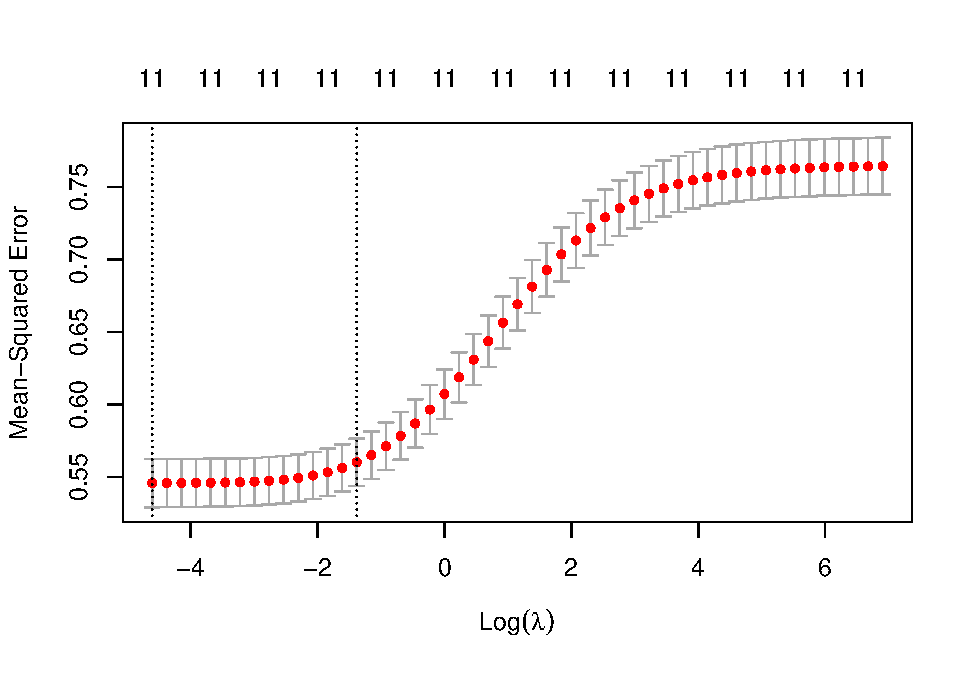
\includegraphics{FinalProject-Bright-Santoro_files/figure-latex/unnamed-chunk-41-1.pdf}
/ The lowest point in the curve indicates the optimal lambda: the log value of lambda that best minimized the error in cross-validation. This can be pulled out of the glmnet output.

\begin{Shaded}
\begin{Highlighting}[]
\NormalTok{opt\_lambda }\OtherTok{\textless{}{-}}\NormalTok{ ridge\_reg}\SpecialCharTok{$}\NormalTok{lambda.min}
\NormalTok{opt\_lambda}
\end{Highlighting}
\end{Shaded}

\begin{verbatim}
## [1] 0.01
\end{verbatim}

\begin{Shaded}
\begin{Highlighting}[]
\NormalTok{ridge\_model }\OtherTok{\textless{}{-}}\NormalTok{ ridge\_reg}\SpecialCharTok{$}\NormalTok{glmnet.fit}
\FunctionTok{summary}\NormalTok{(ridge\_model)}
\end{Highlighting}
\end{Shaded}

\begin{verbatim}
##           Length Class     Mode   
## a0         51    -none-    numeric
## beta      561    dgCMatrix S4     
## df         51    -none-    numeric
## dim         2    -none-    numeric
## lambda     51    -none-    numeric
## dev.ratio  51    -none-    numeric
## nulldev     1    -none-    numeric
## npasses     1    -none-    numeric
## jerr        1    -none-    numeric
## offset      1    -none-    logical
## call        5    -none-    call   
## nobs        1    -none-    numeric
\end{verbatim}

Next, we prepare our test data for prediction.

\begin{Shaded}
\begin{Highlighting}[]
\NormalTok{test.mat }\OtherTok{\textless{}{-}}\NormalTok{ test }\SpecialCharTok{\%\textgreater{}\%} \FunctionTok{select}\NormalTok{(cols) }\SpecialCharTok{\%\textgreater{}\%} \FunctionTok{data.matrix}\NormalTok{()}
\end{Highlighting}
\end{Shaded}

Next, we find the RMSE of the ridge regression.

\begin{Shaded}
\begin{Highlighting}[]
\NormalTok{p}\FloatTok{.4} \OtherTok{\textless{}{-}} \FunctionTok{predict}\NormalTok{(ridge\_model, }\AttributeTok{s =}\NormalTok{ opt\_lambda, }\AttributeTok{newx =}\NormalTok{ test.mat)}

\NormalTok{RMSE}\FloatTok{.4} \OtherTok{\textless{}{-}} \FunctionTok{RMSE}\NormalTok{(p}\FloatTok{.4}\NormalTok{,test}\SpecialCharTok{$}\NormalTok{quality)}
\NormalTok{RMSE}\FloatTok{.4}
\end{Highlighting}
\end{Shaded}

\begin{verbatim}
## [1] 0.7314353
\end{verbatim}

\begin{Shaded}
\begin{Highlighting}[]
\NormalTok{rp}\FloatTok{.4}\OtherTok{\textless{}{-}}\FunctionTok{round}\NormalTok{(p}\FloatTok{.4}\NormalTok{)}
\FunctionTok{mean}\NormalTok{(rp}\FloatTok{.4}\SpecialCharTok{==}\NormalTok{test}\SpecialCharTok{$}\NormalTok{quality)}
\end{Highlighting}
\end{Shaded}

\begin{verbatim}
## [1] 0.5390585
\end{verbatim}

\hypertarget{lasso-regression-1}{%
\section{Lasso Regression}\label{lasso-regression-1}}

The method for LASSO regression is much similar to the above code wise although it is completing something different. Lasso regression, or the Least Absolute Shrinkage and Selection Operator, is also a modification of linear regression. In lasso, the loss function is modified to minimize the complexity of the model by limiting the sum of the absolute values of the model coefficients. \citet{regression_r}

\begin{Shaded}
\begin{Highlighting}[]
\NormalTok{lambdas }\OtherTok{\textless{}{-}} \DecValTok{10}\SpecialCharTok{\^{}}\FunctionTok{seq}\NormalTok{(}\DecValTok{2}\NormalTok{, }\SpecialCharTok{{-}}\DecValTok{3}\NormalTok{, }\AttributeTok{by =} \SpecialCharTok{{-}}\NormalTok{.}\DecValTok{1}\NormalTok{)}

\CommentTok{\# Setting alpha = 1 implements lasso regression}
\NormalTok{lasso\_reg }\OtherTok{\textless{}{-}} \FunctionTok{cv.glmnet}\NormalTok{(train.mat, qual, }\AttributeTok{alpha =} \DecValTok{1}\NormalTok{, }\AttributeTok{lambda =}\NormalTok{ lambdas)}
\FunctionTok{plot}\NormalTok{(lasso\_reg)}
\end{Highlighting}
\end{Shaded}

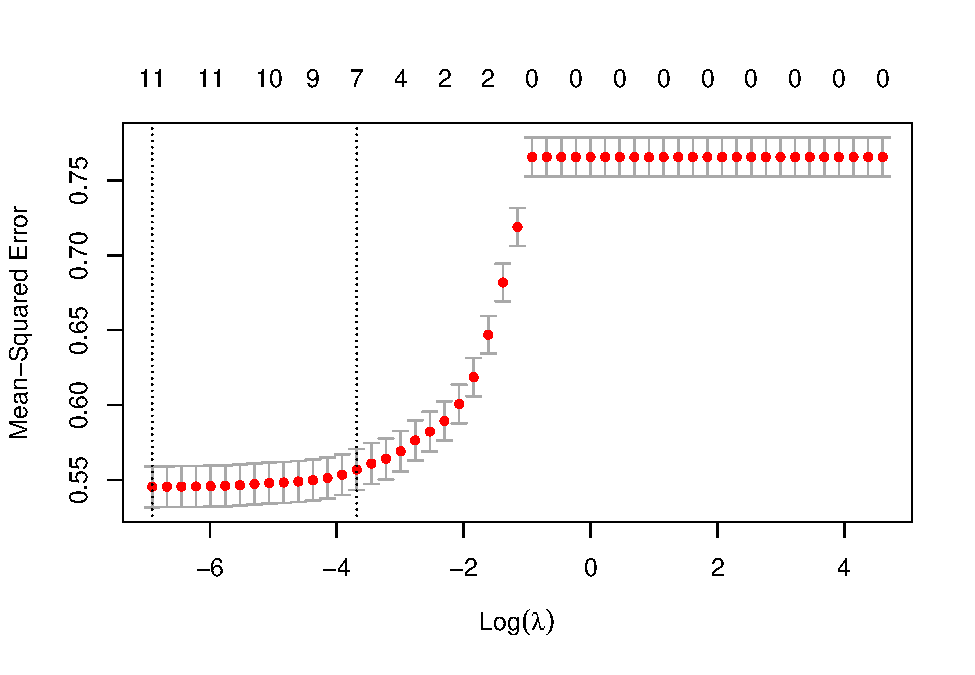
\includegraphics{FinalProject-Bright-Santoro_files/figure-latex/unnamed-chunk-47-1.pdf}

\begin{Shaded}
\begin{Highlighting}[]
\CommentTok{\# Best }
\NormalTok{lambda\_best }\OtherTok{\textless{}{-}}\NormalTok{ lasso\_reg}\SpecialCharTok{$}\NormalTok{lambda.min }
\NormalTok{lambda\_best}
\end{Highlighting}
\end{Shaded}

\begin{verbatim}
## [1] 0.001
\end{verbatim}

\begin{Shaded}
\begin{Highlighting}[]
\NormalTok{p}\FloatTok{.5} \OtherTok{\textless{}{-}} \FunctionTok{predict}\NormalTok{(lasso\_reg, }\AttributeTok{s =}\NormalTok{ lambda\_best, }\AttributeTok{newx =}\NormalTok{ test.mat)}

\NormalTok{RMSE}\FloatTok{.5} \OtherTok{\textless{}{-}} \FunctionTok{RMSE}\NormalTok{(p}\FloatTok{.5}\NormalTok{,test}\SpecialCharTok{$}\NormalTok{quality)}
\NormalTok{RMSE}\FloatTok{.5}
\end{Highlighting}
\end{Shaded}

\begin{verbatim}
## [1] 0.7315071
\end{verbatim}

\begin{Shaded}
\begin{Highlighting}[]
\NormalTok{rp}\FloatTok{.5}\OtherTok{\textless{}{-}}\FunctionTok{round}\NormalTok{(p}\FloatTok{.5}\NormalTok{)}
\FunctionTok{mean}\NormalTok{(rp}\FloatTok{.5}\SpecialCharTok{==}\NormalTok{test}\SpecialCharTok{$}\NormalTok{quality)}
\end{Highlighting}
\end{Shaded}

\begin{verbatim}
## [1] 0.5395758
\end{verbatim}

\hypertarget{features-of-the-glmnet-package}{%
\subsection{Features of the `glmnet' Package}\label{features-of-the-glmnet-package}}

\(\lambda\) is defined once and \(\alpha\) where lasso is scaled by \(\alpha\) and ridge penalty is scaled by \((1-\alpha\)).

\hypertarget{elastic-net-regression}{%
\subsection{Elastic Net Regression}\label{elastic-net-regression}}

Elastic net regression combines the properties of ridge and lasso regression. So, we need a technique to cycle through find the most optimal limiting factors.The first line of code creates a training control object train\_cont which specifies how the repeated cross validation will take place. The second line builds the elastic regression model in which a range of possible alpha and lambda values are tested and their optimum value is selected. \citet{regression_r}

\begin{verbatim}
## Warning in nominalTrainWorkflow(x = x, y = y, wts = weights, info = trainInfo, :
## There were missing values in resampled performance measures.
\end{verbatim}

\begin{Shaded}
\begin{Highlighting}[]
\CommentTok{\# Best tuning parameter}
\NormalTok{elastic\_reg}\SpecialCharTok{$}\NormalTok{bestTune}
\end{Highlighting}
\end{Shaded}

\begin{verbatim}
##       alpha      lambda
## 6 0.8902916 0.001641559
\end{verbatim}

\begin{Shaded}
\begin{Highlighting}[]
\NormalTok{elastic\_reg }\OtherTok{\textless{}{-}} \FunctionTok{glmnet}\NormalTok{(train.mat , qual, }\AttributeTok{alpha =}\NormalTok{ elastic\_reg}\SpecialCharTok{$}\NormalTok{bestTune[}\DecValTok{1}\NormalTok{,}\DecValTok{1}\NormalTok{], }\AttributeTok{lambda =}\NormalTok{ elastic\_reg}\SpecialCharTok{$}\NormalTok{bestTune[}\DecValTok{1}\NormalTok{,}\DecValTok{2}\NormalTok{])}
\end{Highlighting}
\end{Shaded}

\begin{Shaded}
\begin{Highlighting}[]
\NormalTok{p}\FloatTok{.6} \OtherTok{\textless{}{-}} \FunctionTok{predict}\NormalTok{(elastic\_reg, }\AttributeTok{s =}\NormalTok{ elastic\_reg}\SpecialCharTok{$}\NormalTok{bestTune, }\AttributeTok{newx =}\NormalTok{ test.mat)}

\NormalTok{RMSE}\FloatTok{.6} \OtherTok{\textless{}{-}} \FunctionTok{RMSE}\NormalTok{(p}\FloatTok{.6}\NormalTok{,test}\SpecialCharTok{$}\NormalTok{quality)}
\NormalTok{RMSE}\FloatTok{.6}
\end{Highlighting}
\end{Shaded}

\begin{verbatim}
## [1] 0.7314186
\end{verbatim}

\begin{Shaded}
\begin{Highlighting}[]
\NormalTok{rp}\FloatTok{.6}\OtherTok{\textless{}{-}}\FunctionTok{round}\NormalTok{(p}\FloatTok{.6}\NormalTok{)}
\NormalTok{acc}\FloatTok{.6} \OtherTok{\textless{}{-}} \FunctionTok{mean}\NormalTok{(rp}\FloatTok{.6}\SpecialCharTok{==}\NormalTok{test}\SpecialCharTok{$}\NormalTok{quality)}
\end{Highlighting}
\end{Shaded}

\begin{Shaded}
\begin{Highlighting}[]
\NormalTok{accuracy[}\DecValTok{3}\NormalTok{,}\DecValTok{1}\NormalTok{] }\OtherTok{\textless{}{-}}\NormalTok{ acc}\FloatTok{.6}
\end{Highlighting}
\end{Shaded}

\hypertarget{results}{%
\chapter{Results}\label{results}}

\begin{Shaded}
\begin{Highlighting}[]
\NormalTok{accuracy}
\end{Highlighting}
\end{Shaded}

\begin{verbatim}
##                Accuracy
## K-Nearest     0.5628557
## Random Forest 0.6844283
## Regression    0.5380238
\end{verbatim}

We have concluded from our research that Random Forest provides the most accurate predictions of quality for this dataset of wine samples. We believe that additional tuning to the Random Forest model parameters and a larger dataset for training our model could help to increase the level of accuracy in our predictions in the future.

\hypertarget{references}{%
\chapter{References}\label{references}}

P. Cortez, A. Cerdeira, F. Almeida, T. Matos and J. Reis.
Modeling wine preferences by data mining from physiochemical properties. In Decision Support Systems, Elsevier, 47(4):547-553, 2009.

Puckette, Madeline. ``What Is Wine Exactly?'' Wine Folly, 5 Oct.~2015, winefolly.com/deep-dive/what-is-wine.

``Descriptive Statistics.'' Wikipedia, en.wikipedia.org/wiki/Descriptive\_statistics. Accessed 29 May 2021.

``Linear, Lasso, and Ridge Regression with R'' Deepika Singh, 12 Nov.~2019, \url{https://www.pluralsight.com/guides/linear-lasso-and-ridge-regression-with-r}

``Ridge Regression, LASSO, and Elastic Nets'' Derek Kane, 23, Feb.~2015, \url{https://www.slideshare.net/DerekKane/data-science-part-xii-ridge-regression-lasso-and-elastic-nets}; \url{https://www.youtube.com/watch?v=ipb2MhSRGdw}

Stephanie Glen. ``RMSE: Root Mean Square Error'' From StatisticsHowTo.com: Elementary Statistics for the rest of us! \url{https://www.statisticshowto.com/probability-and-statistics/regression-analysis/rmse-root-mean-square-error/}

Breiman, Leo, and Adele Cutler. ``Random Forests.'' Berkeley Statistics, www.stat.berkeley.edu/\textasciitilde breiman/RandomForests/cc\_home.htm. Accessed 30 May 2021.

  \bibliography{book.bib}

\end{document}
